\chapter{Módulo 3: Leds y sensores digitales}

Si tiene instalado el microcontrolador, removerlo del zócalo

\section{Paso 1:}

Instalar resistencias faltantes. R1 a R8

\begin{figure}[h]
	\centering
	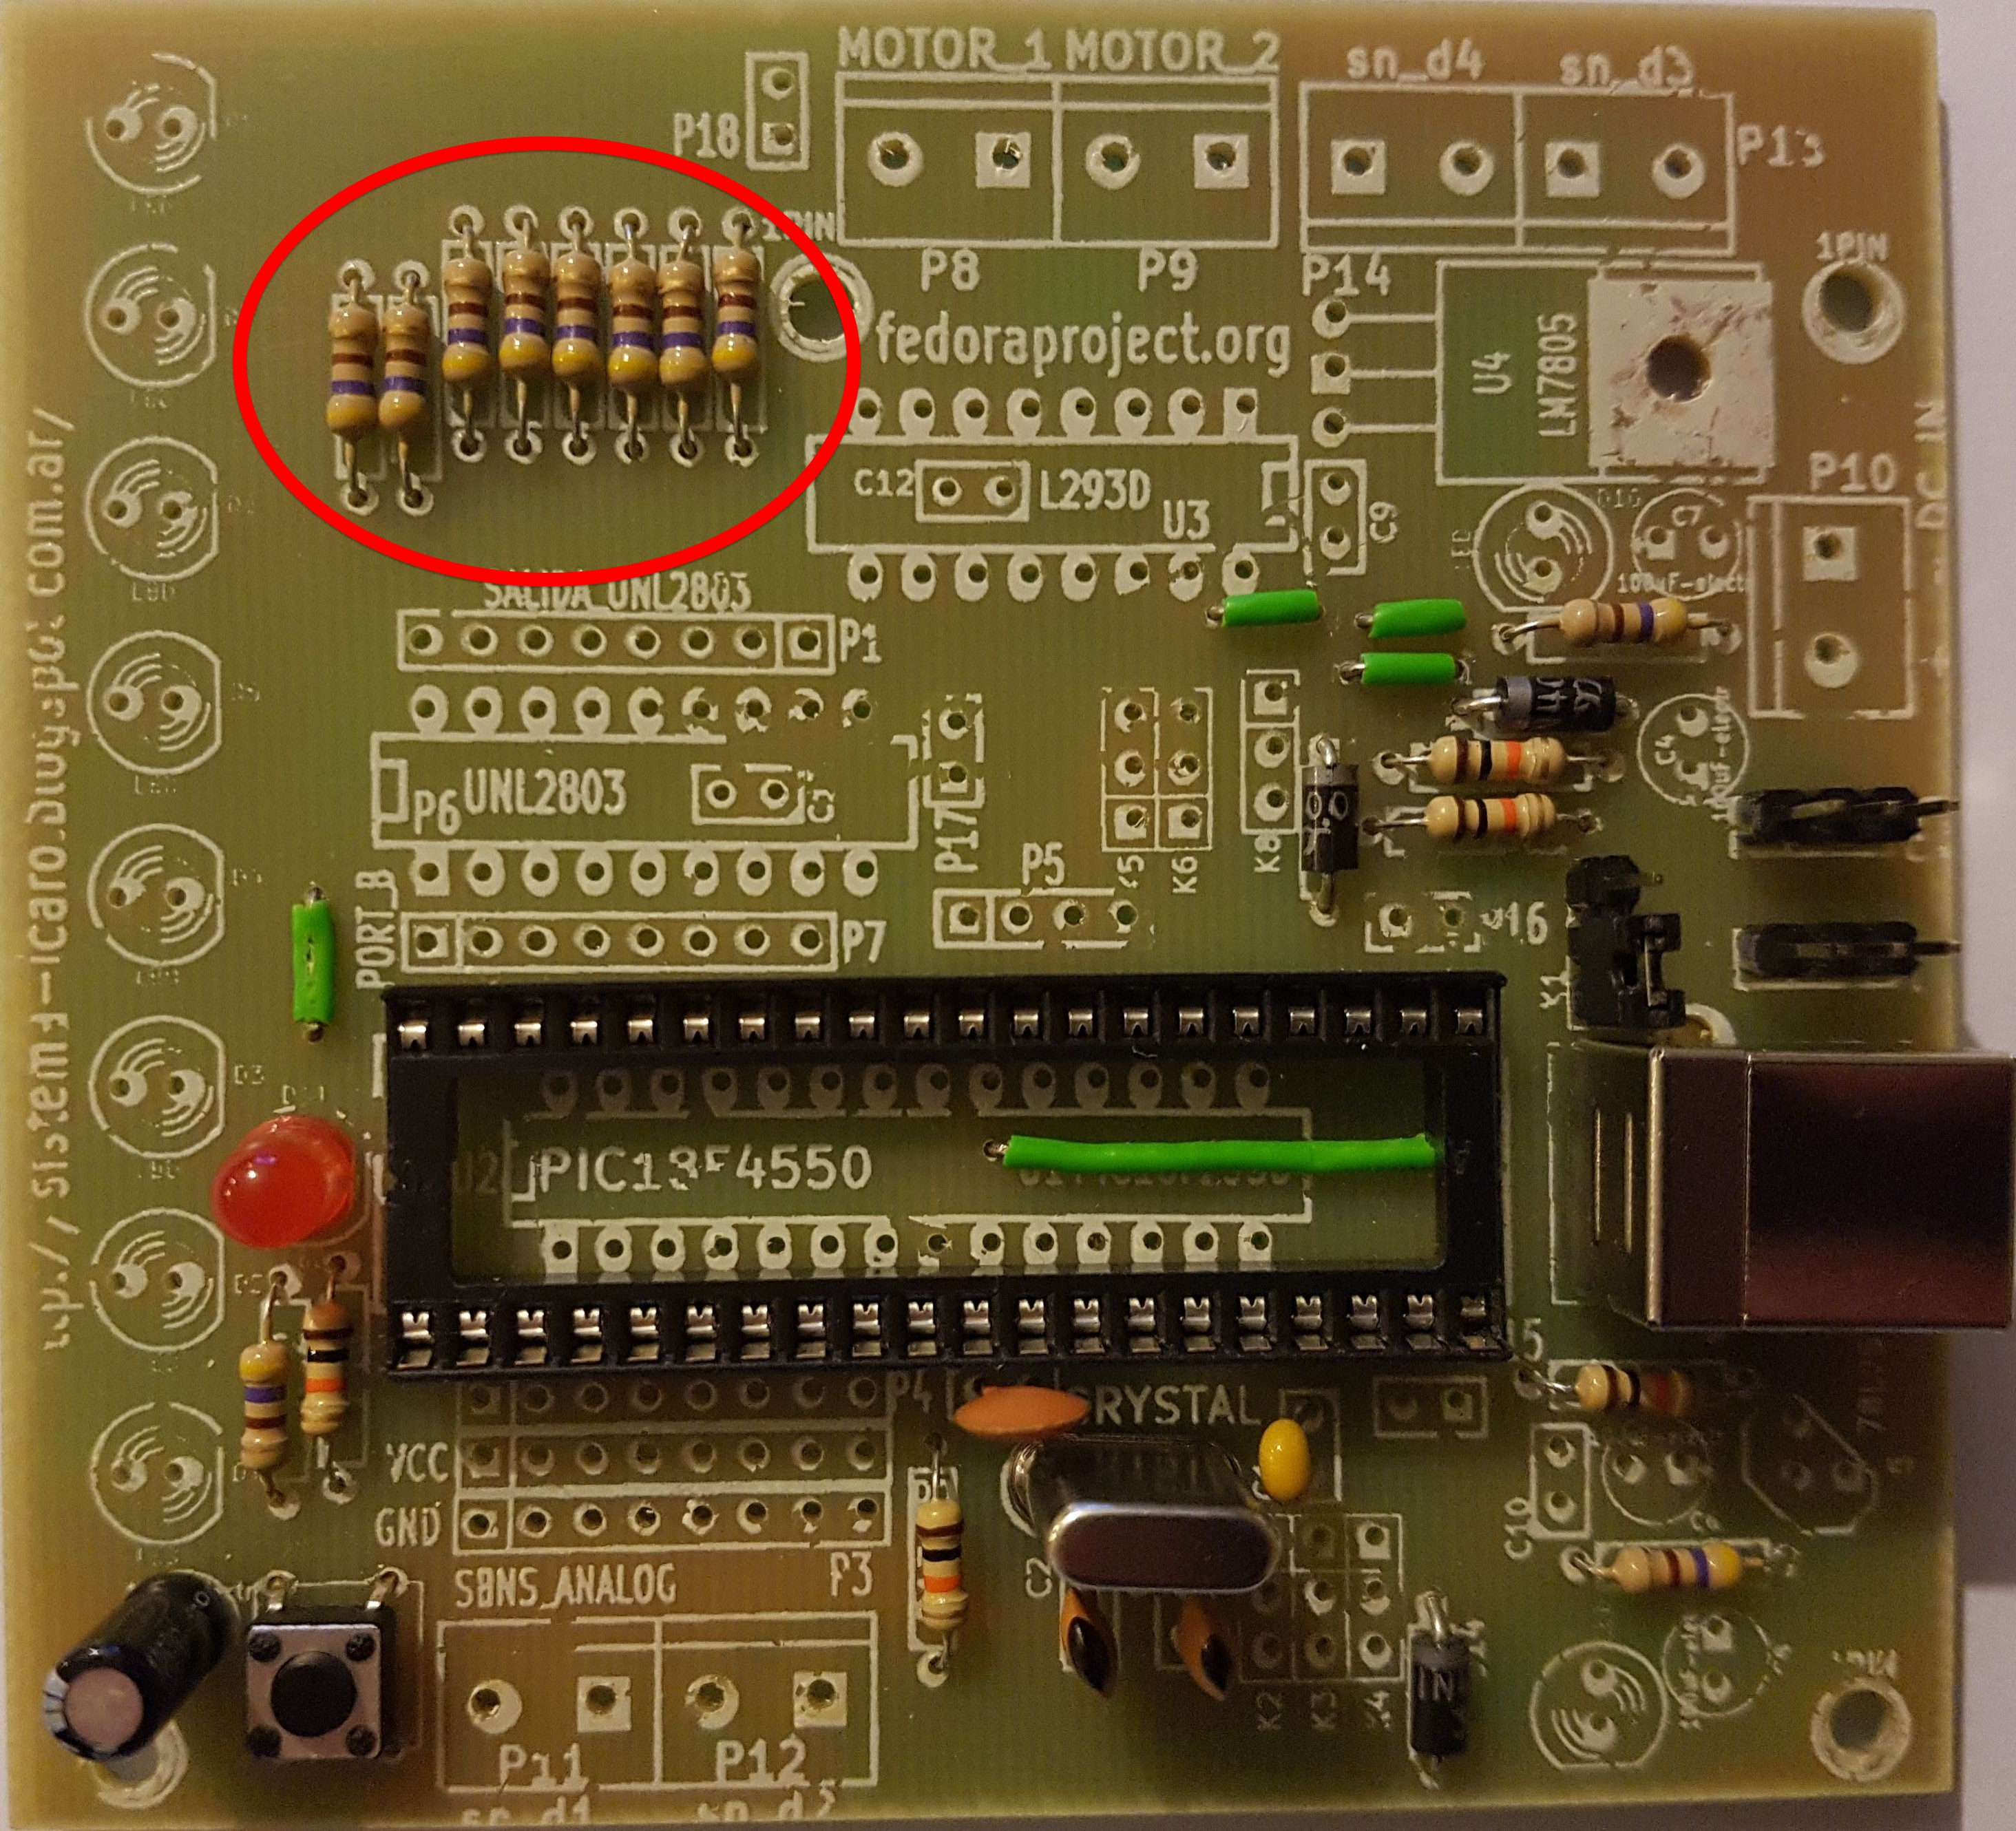
\includegraphics[width=0.8\linewidth]{Modulo_3/M3_1}
	\caption{Módulo 3 - Paso 1}
	\label{fig:M3_1}
\end{figure}

\newpage

\section{Paso 2:}

Instalar capacitor cerámico 0.1uF C13

\begin{figure}[h]
	\centering
	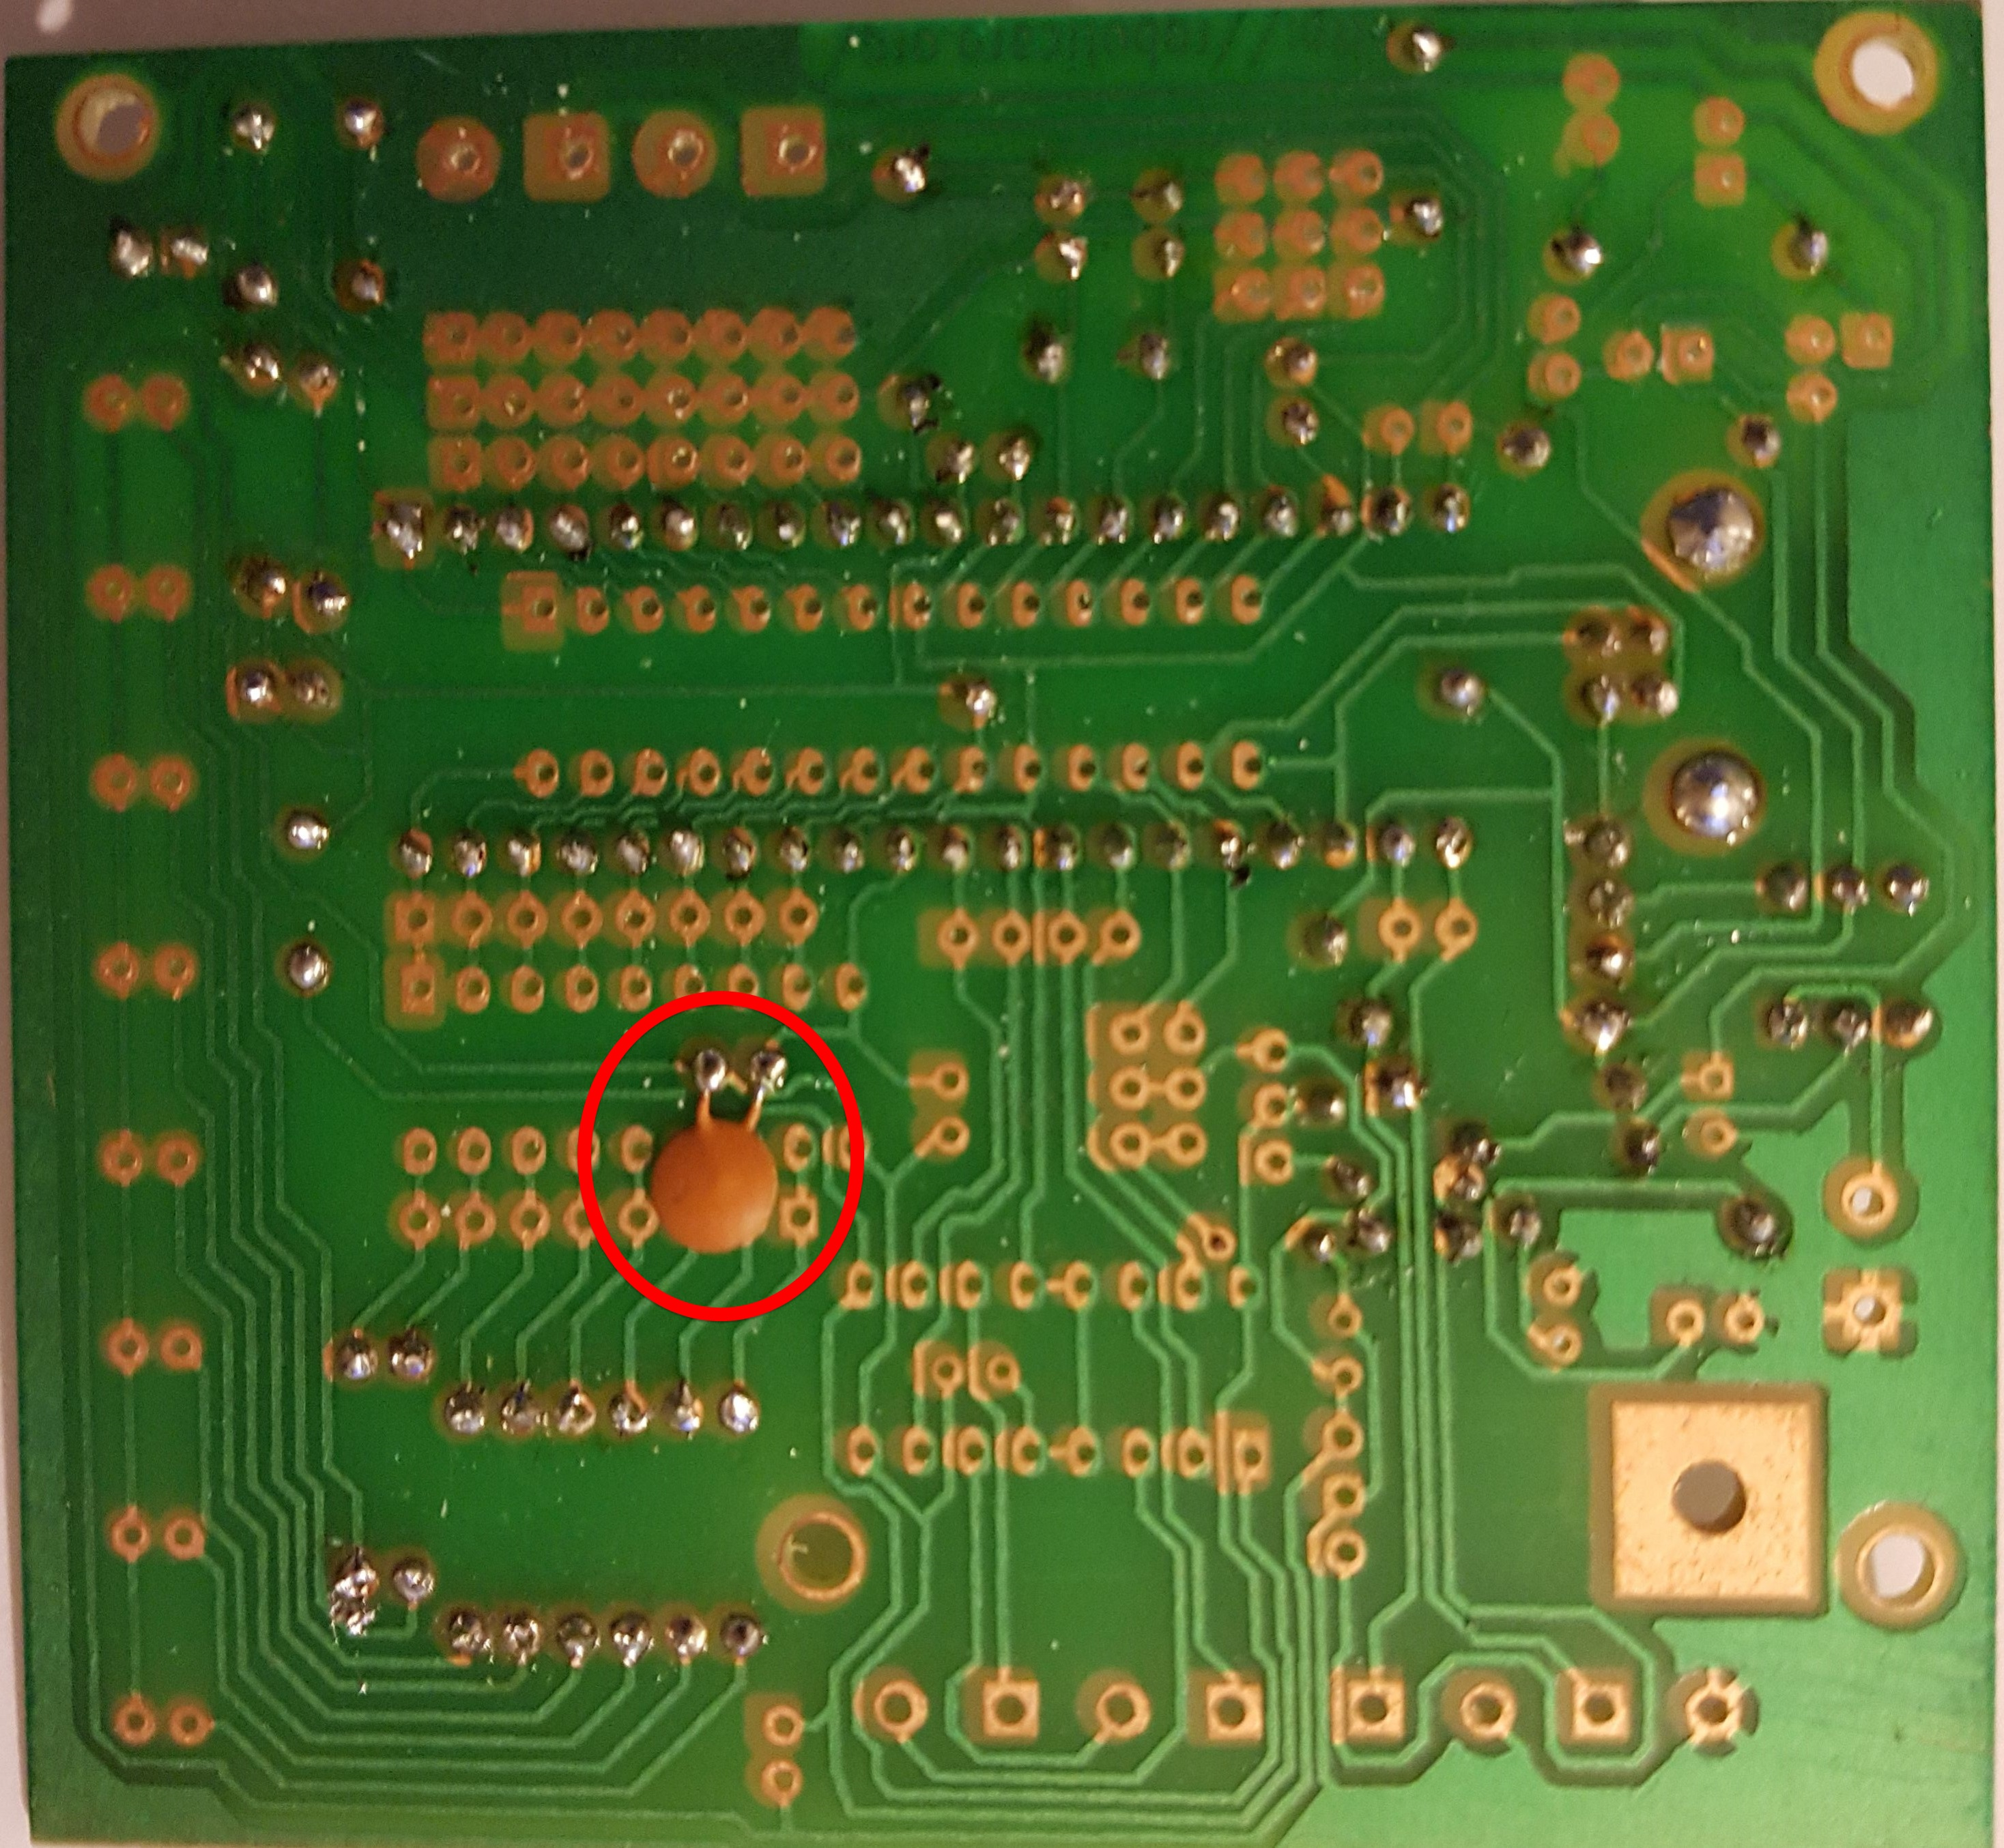
\includegraphics[width=0.8\linewidth]{Modulo_3/M3_2}
	\caption{Módulo 3 - Paso 2}
	\label{fig:M3_2}
\end{figure}

\newpage

\section{Paso 3:}

Instalar zócalo de 18 patas (9x2) P6 Tomar en cuenta alinear la muesca del diagrama de la placa con la muesca del zócalo.

\begin{figure}[h]
	\centering
	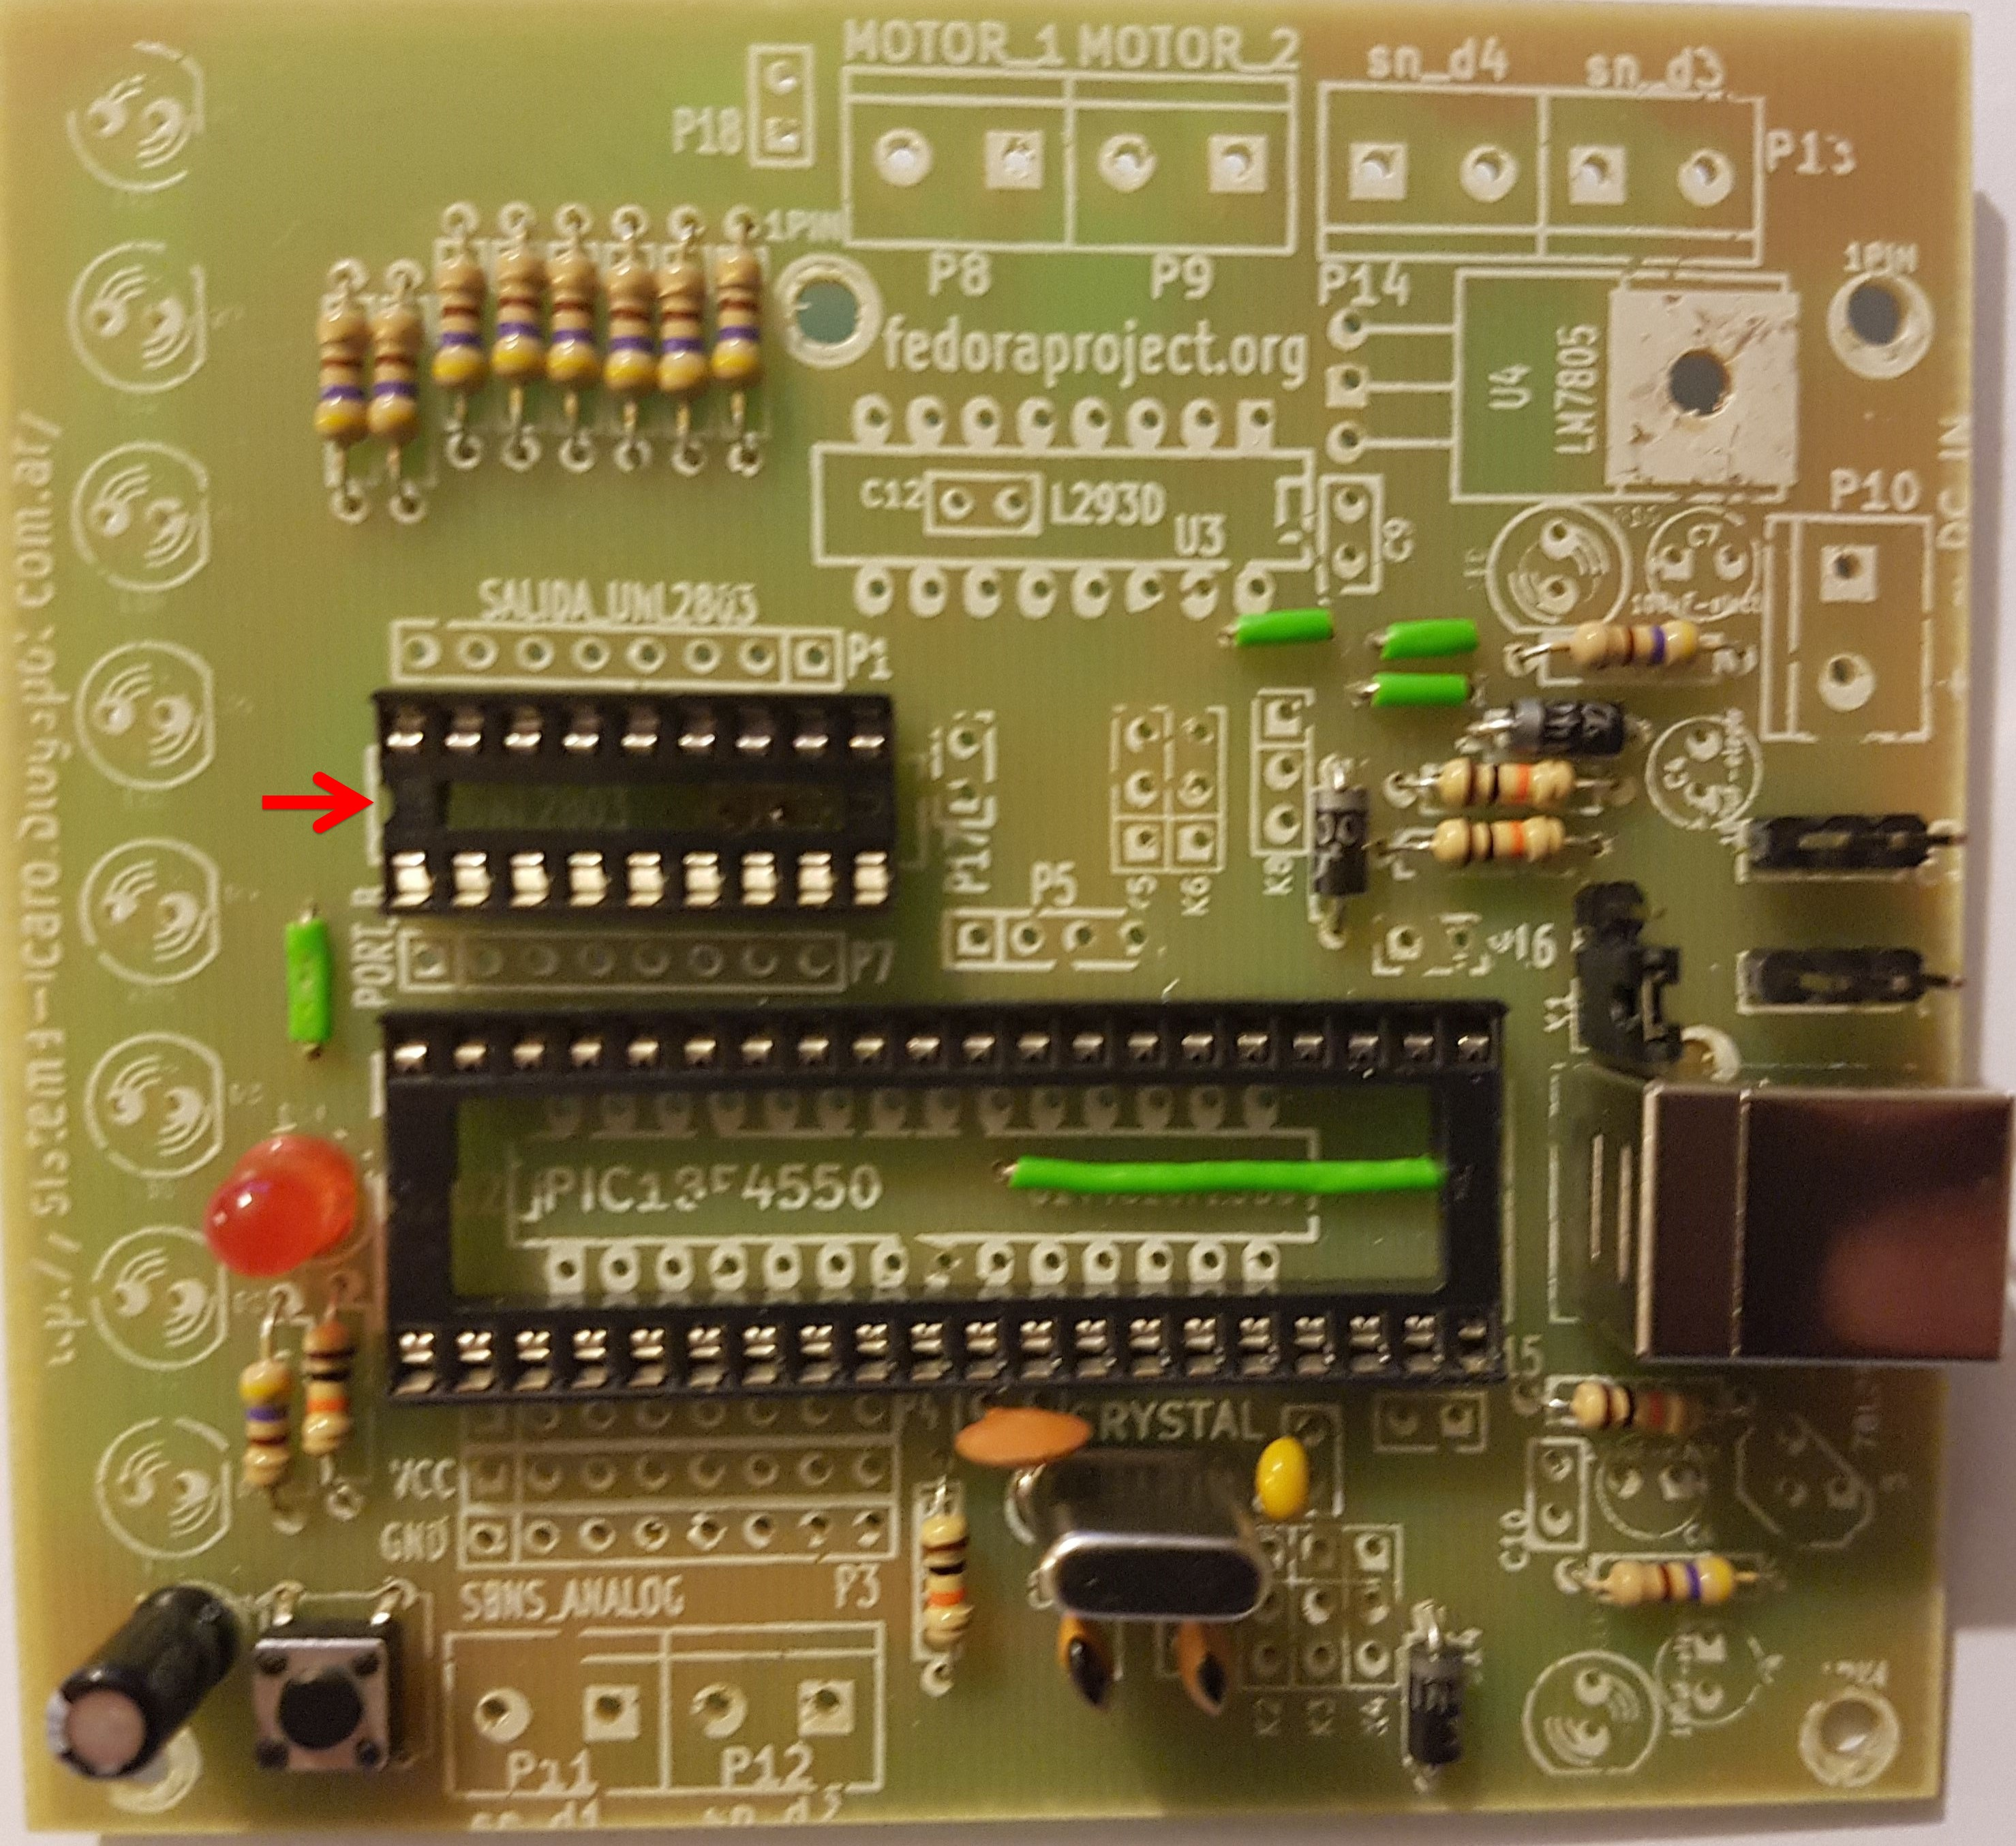
\includegraphics[width=0.8\linewidth]{Modulo_3/M3_3}
	\caption{Módulo 3 - Paso 3}
	\label{fig:M3_3}
\end{figure}

\newpage

\section{Paso 4:}

Instalar pines hembras (Port B) P7

\begin{figure}[h]
	\centering
	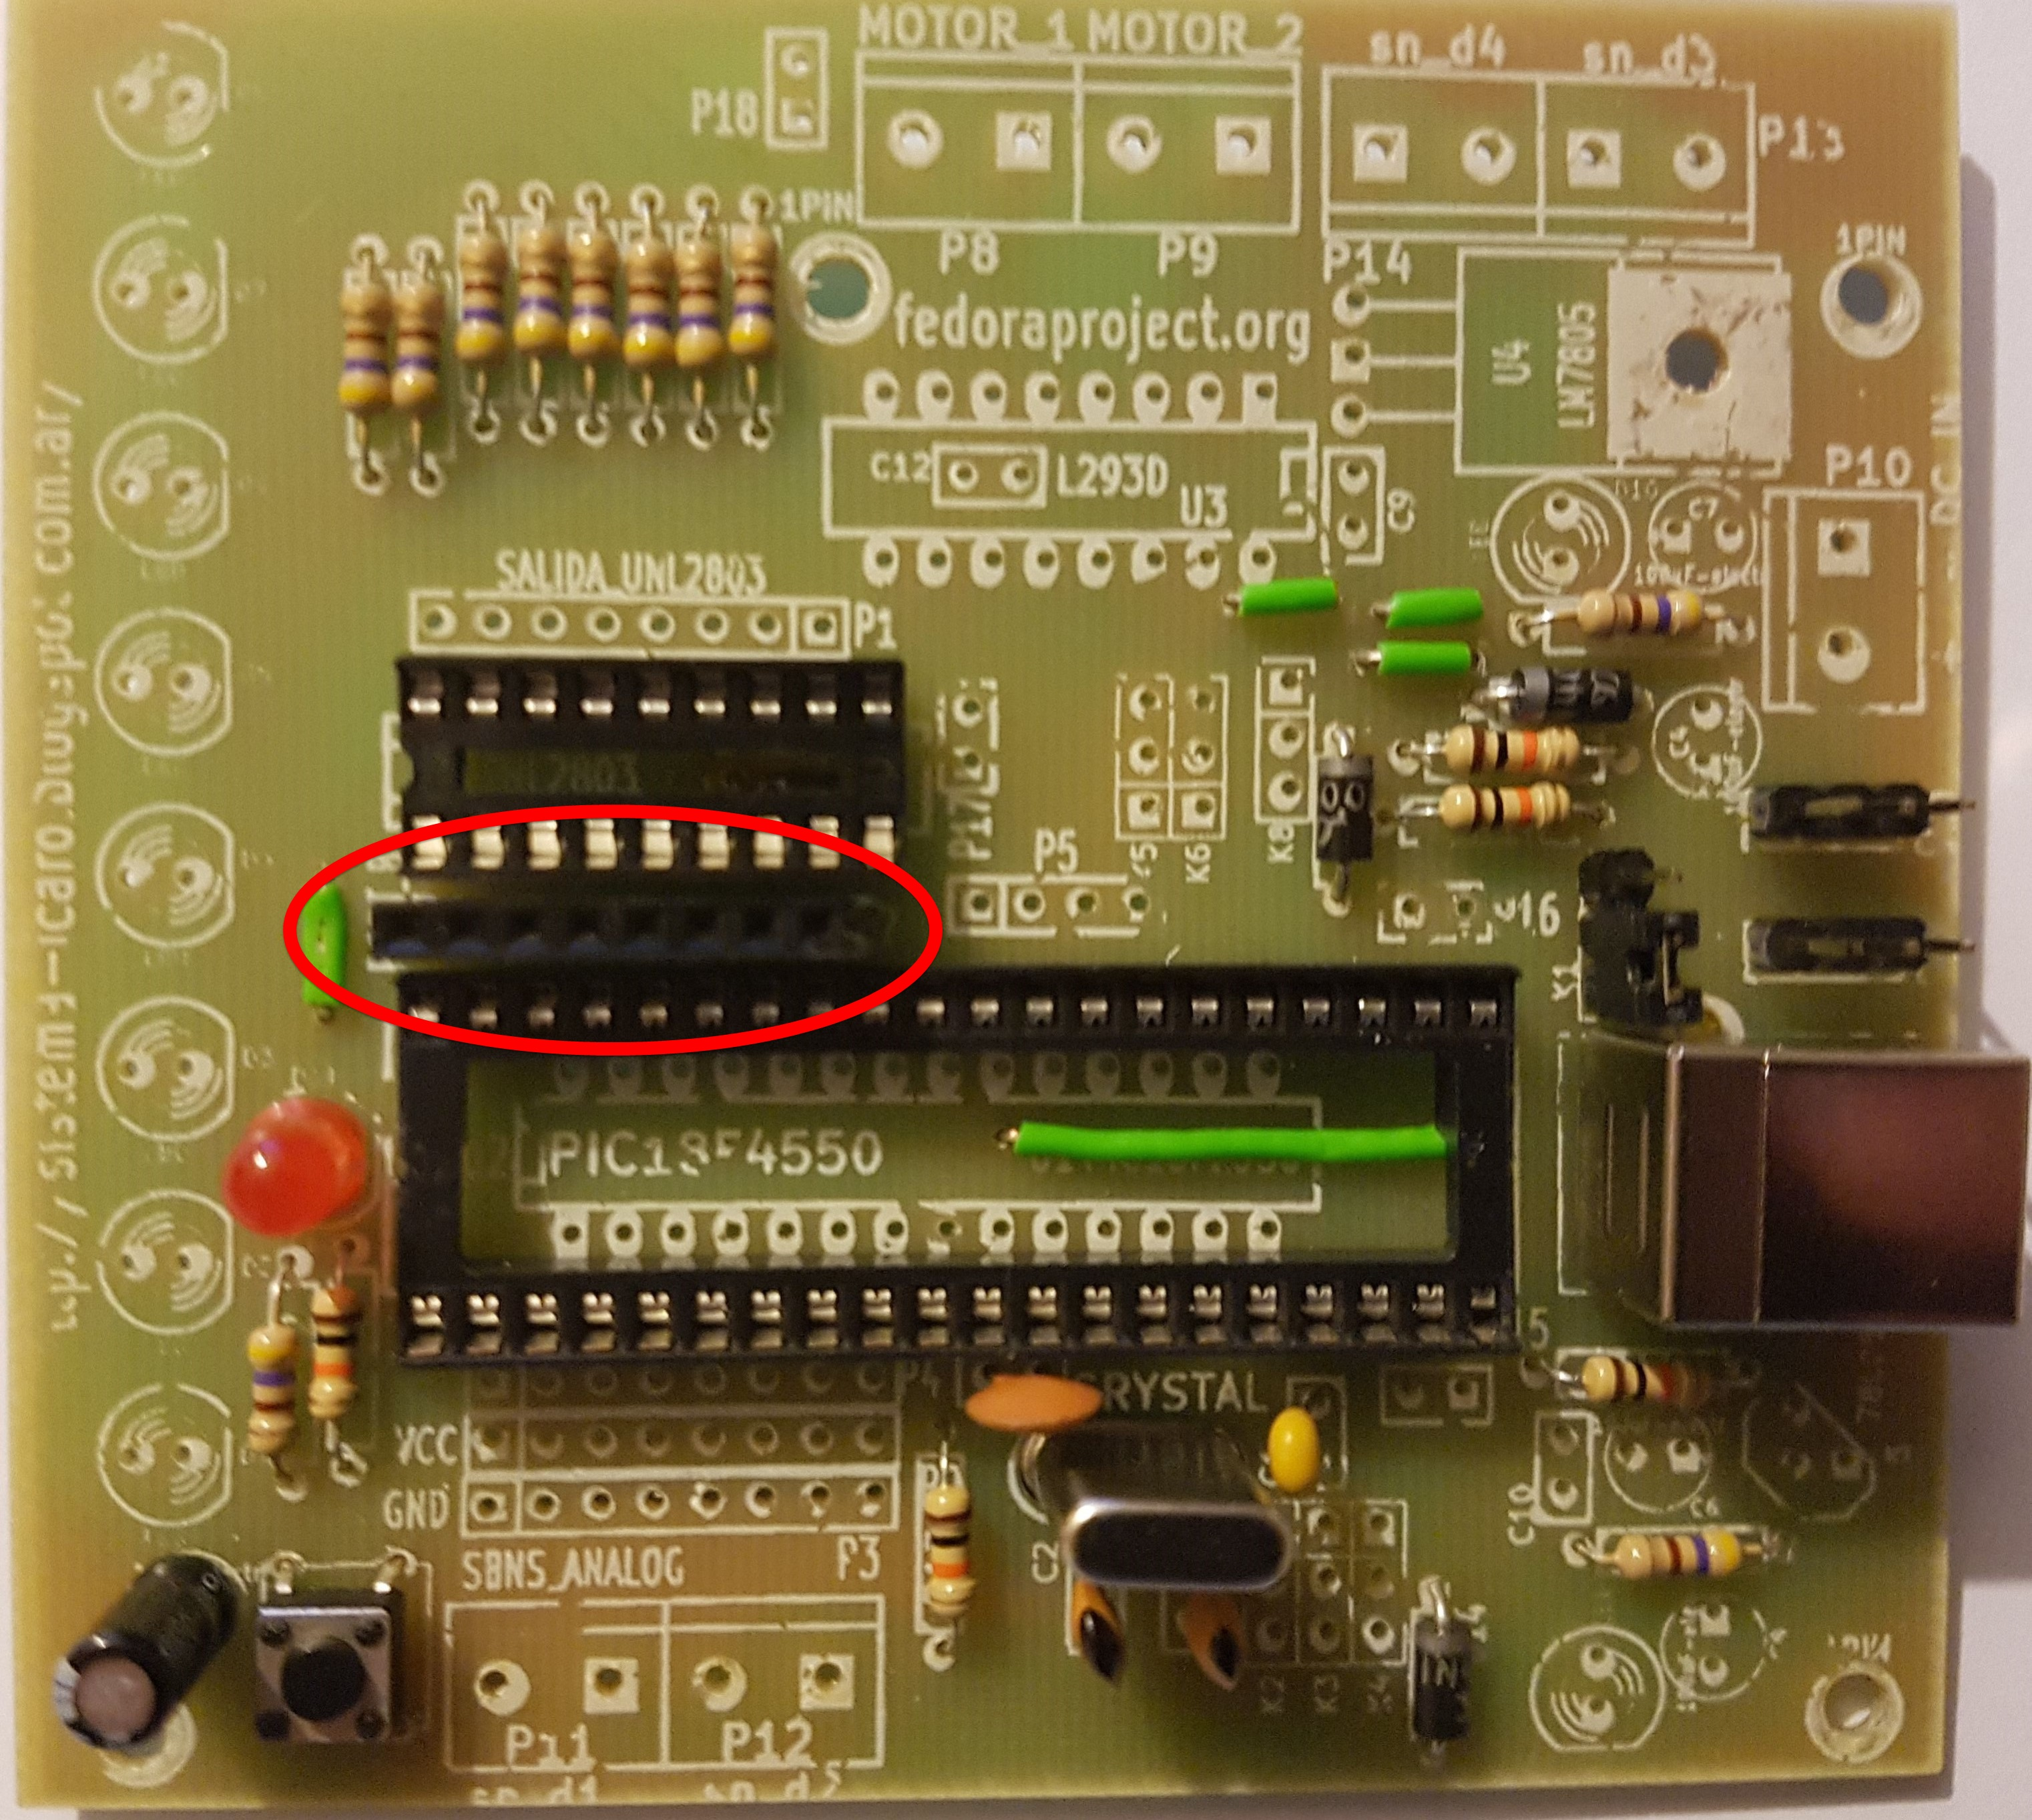
\includegraphics[width=0.8\linewidth]{Modulo_3/M3_4}
	\caption{Módulo 3 - Paso 4}
	\label{fig:M3_4}
\end{figure}

\newpage
\section{Paso 5:}

Instalar pines hembras P1

\begin{figure}[h]
	\centering
	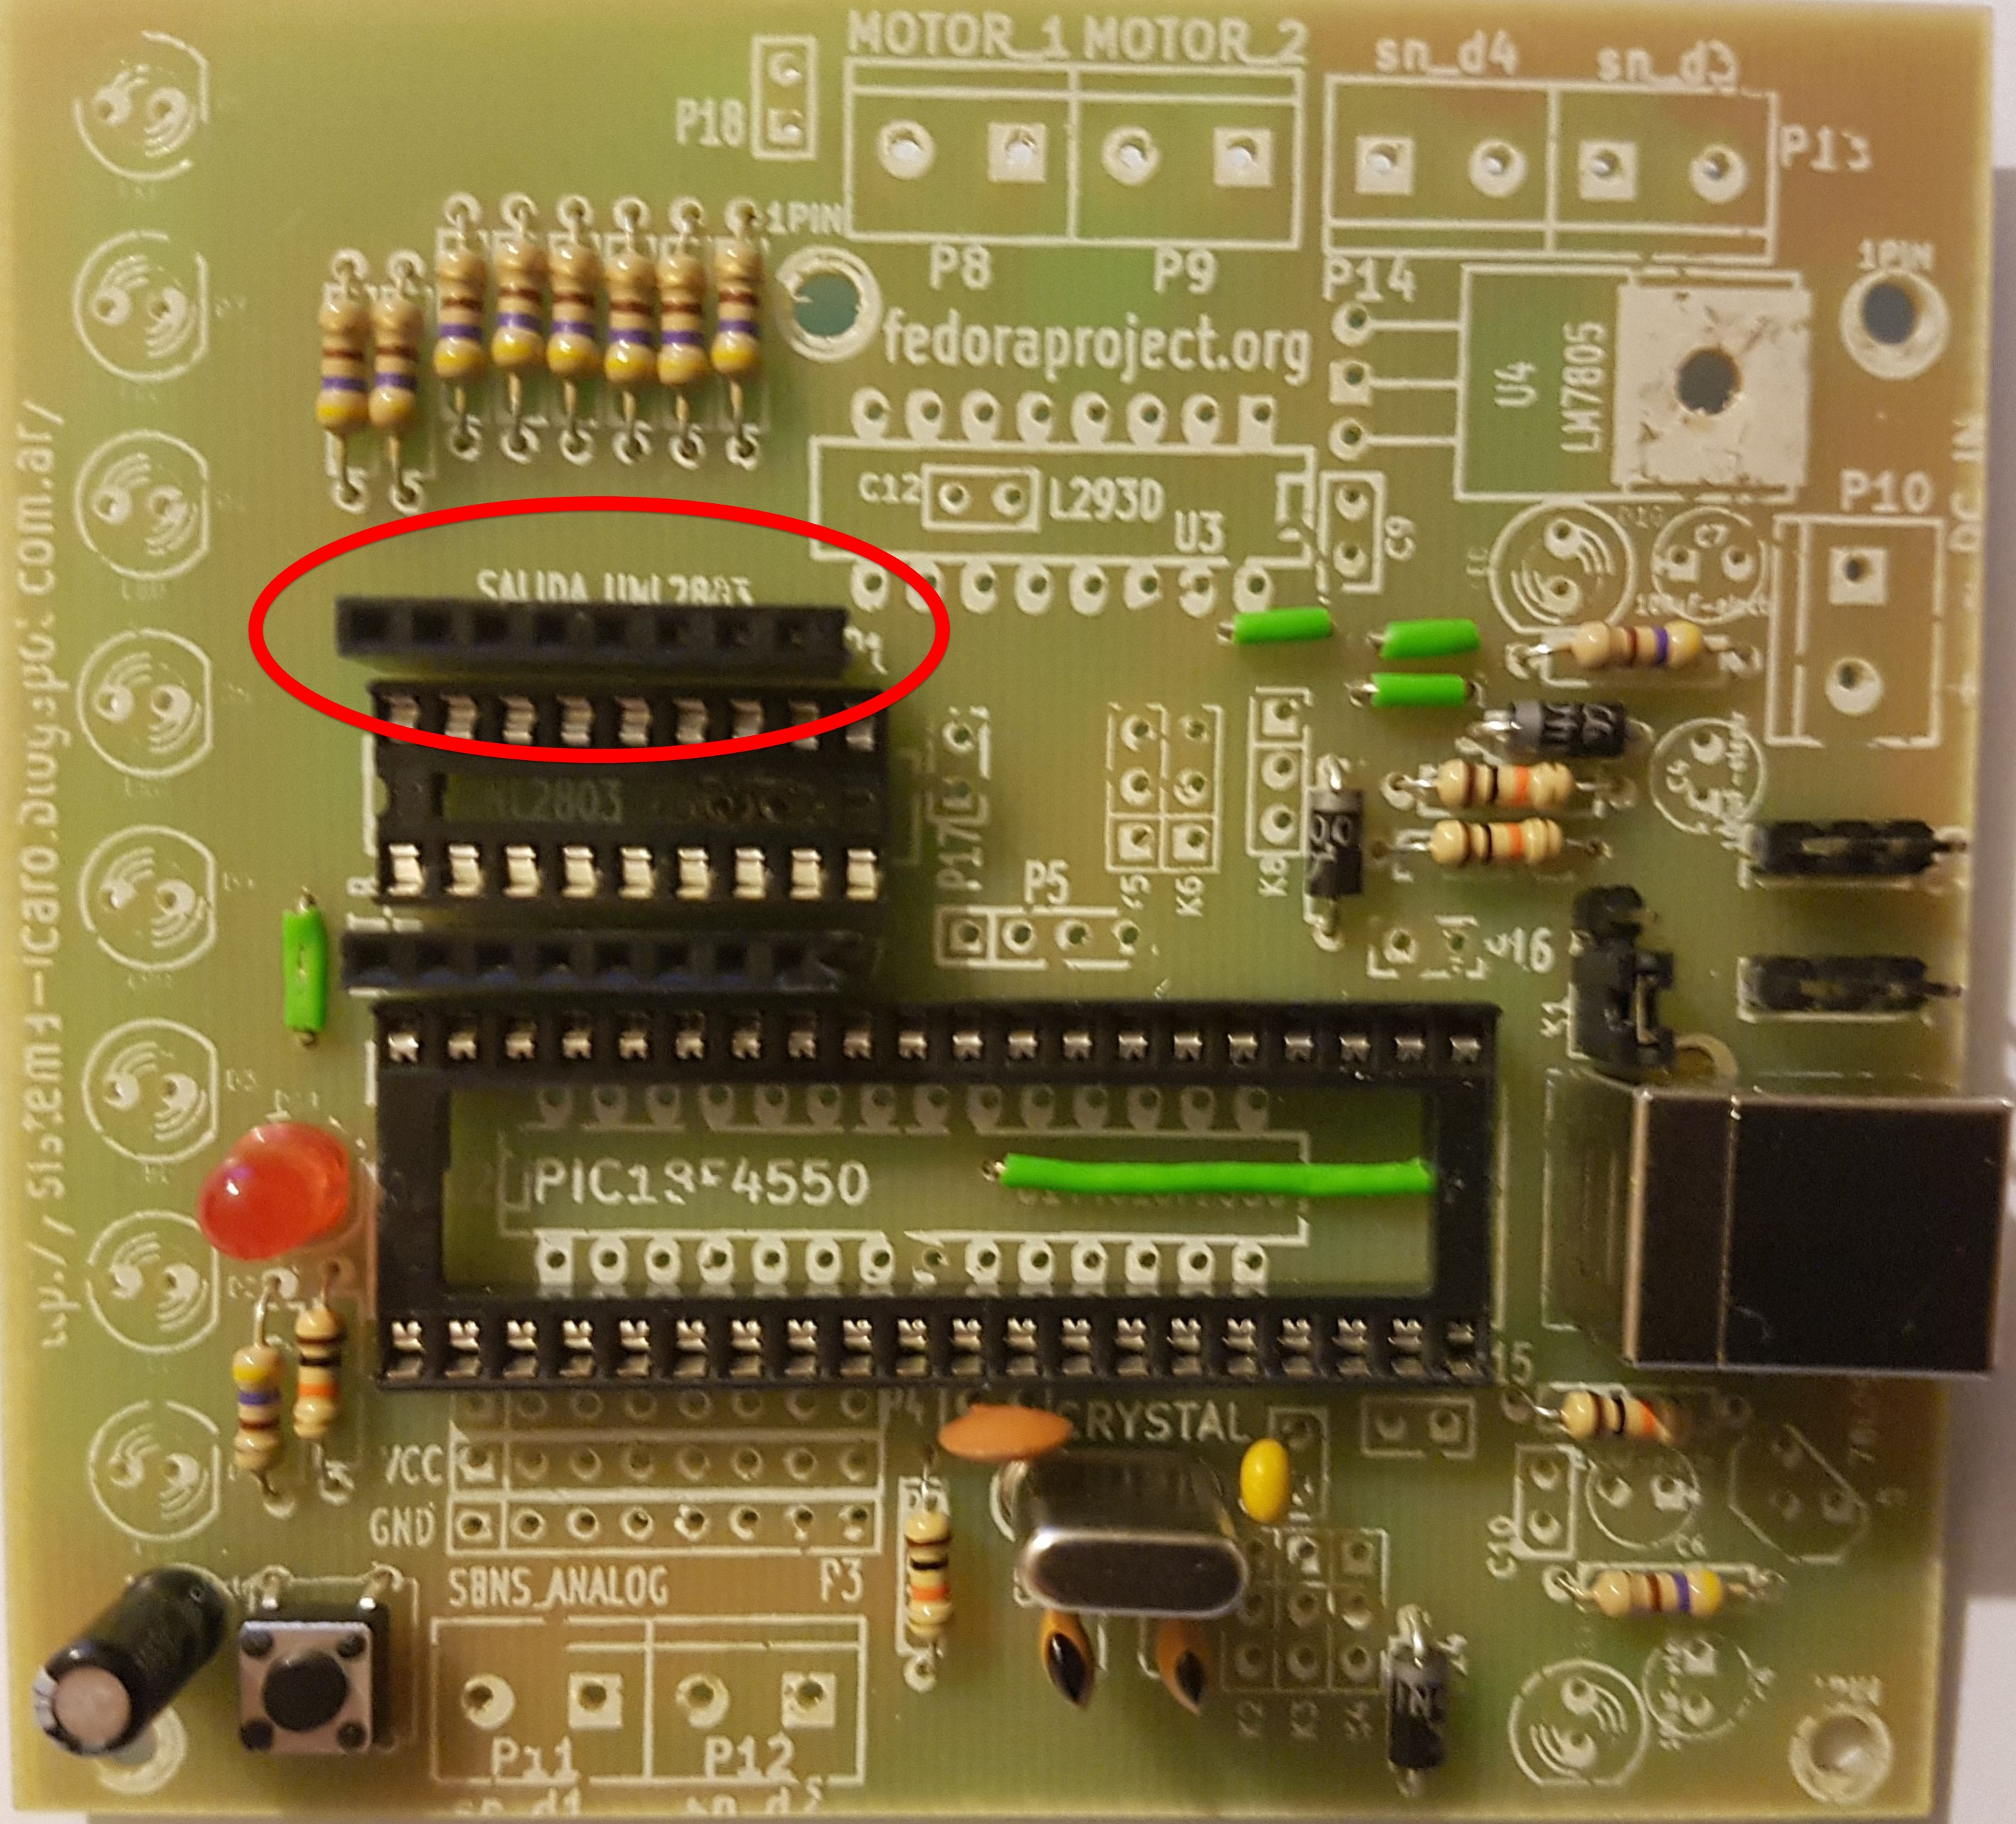
\includegraphics[width=0.8\linewidth]{Modulo_3/M3_5}
	\caption{Módulo 3 - Paso 5}
	\label{fig:M3_5}
\end{figure}

\newpage

\section{Paso 6:}

Instalar leds de la barra de indicación. D1 a D8. Se recomienda todos del mismo color.

\begin{figure}[h]
	\centering
	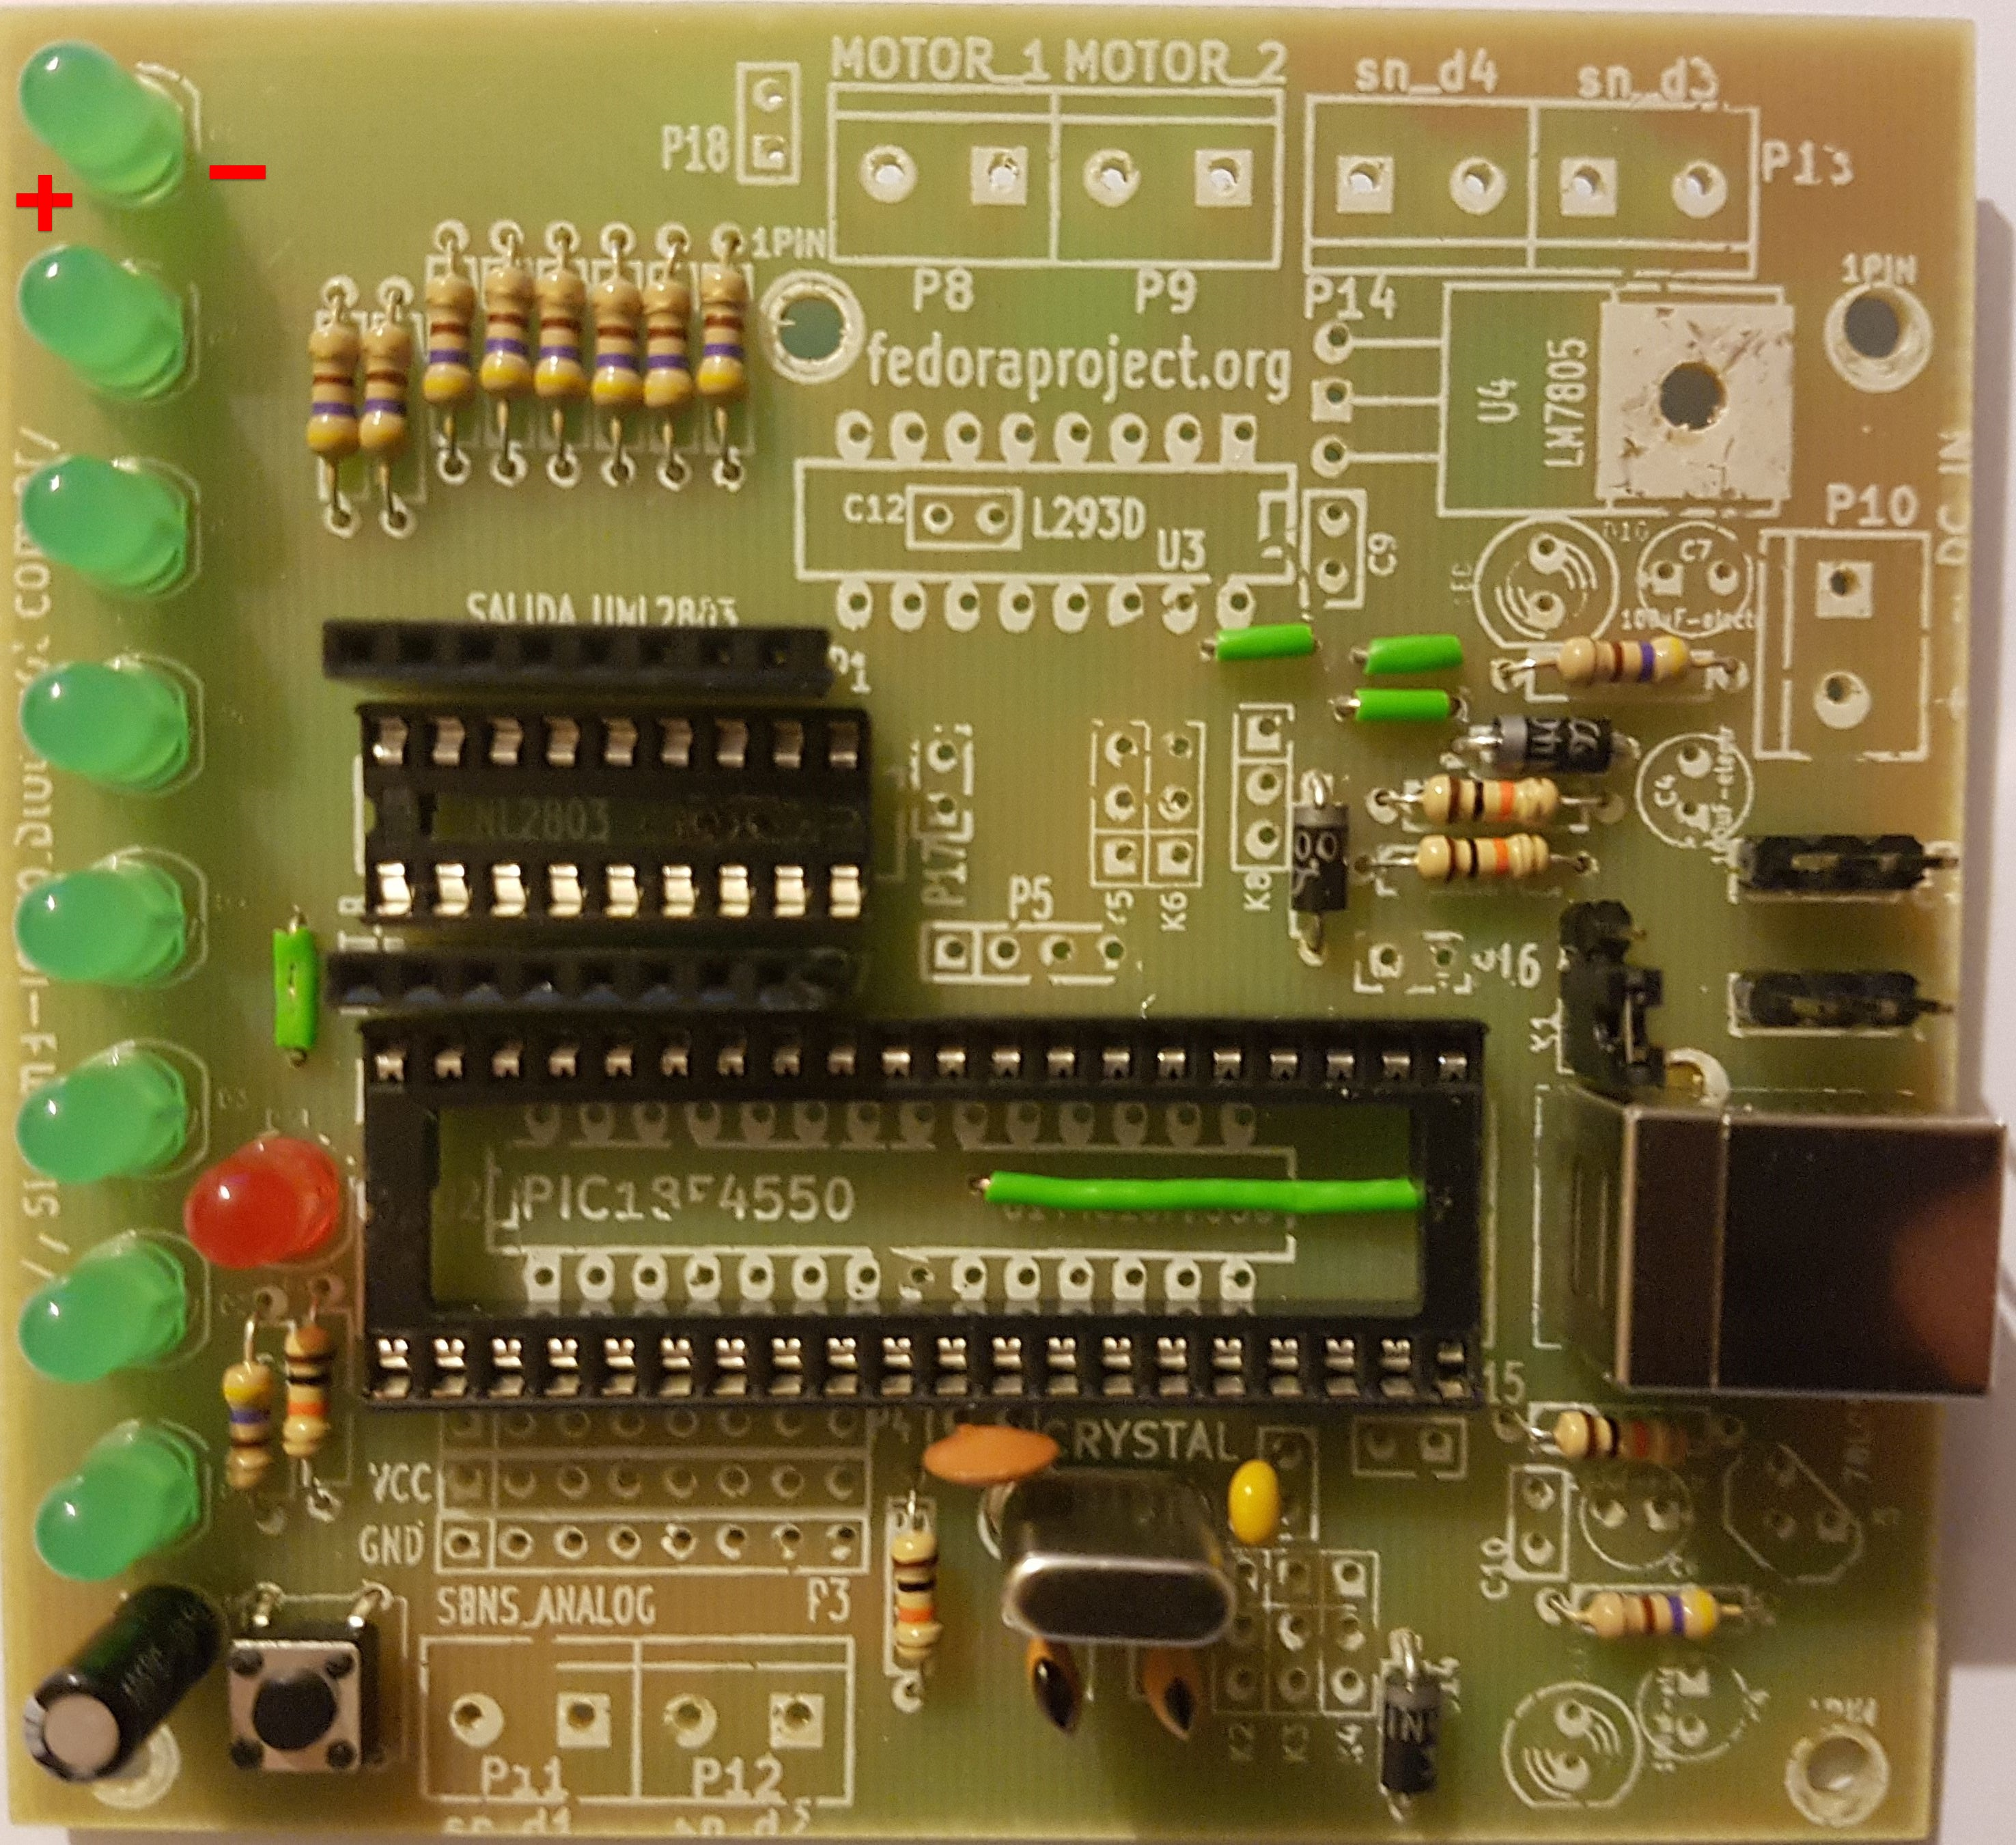
\includegraphics[width=0.8\linewidth]{Modulo_3/M3_6}
	\caption{Módulo 3 - Paso 6}
	\label{fig:M3_6}
\end{figure}

\newpage

\section{Paso 7:}

Instalar pines hembras P15 (Se puede usar como entrada de P11 y P12)

\begin{figure}[h]
	\centering
	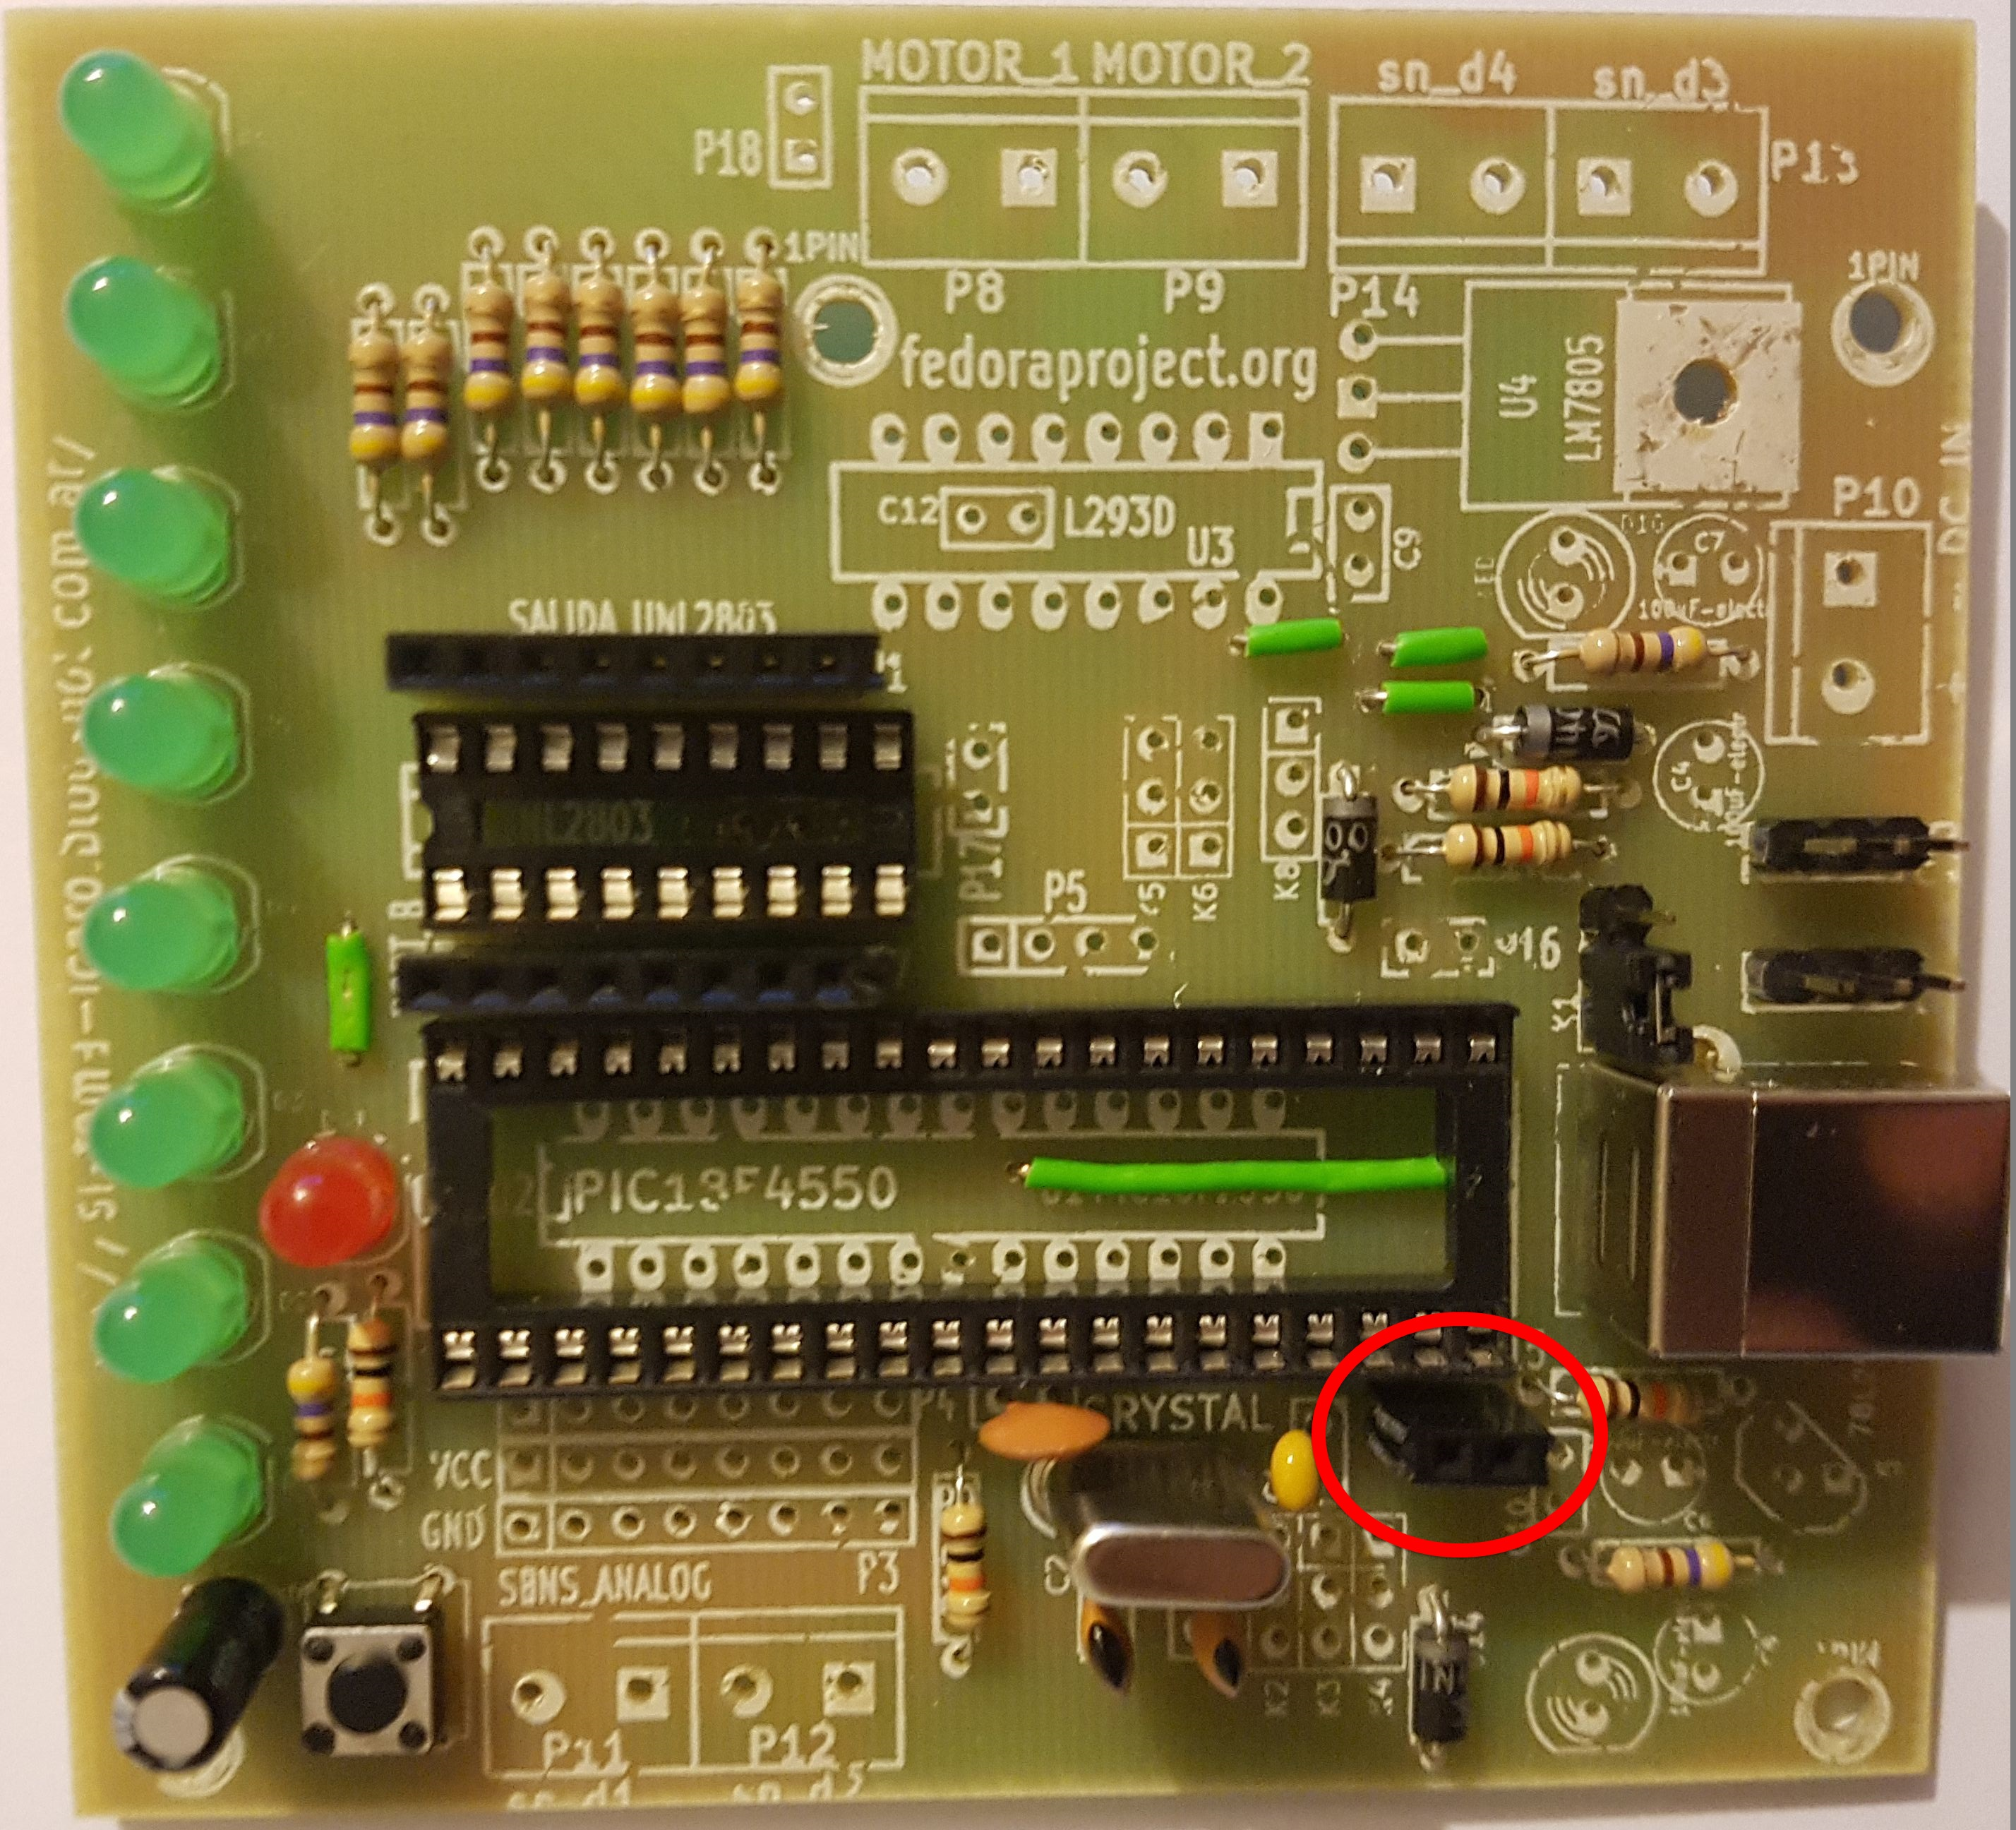
\includegraphics[width=0.8\linewidth]{Modulo_3/M3_7}
	\caption{Módulo 3 - Paso 7}
	\label{fig:M3_7}
\end{figure}

\newpage

\section{Paso 8:}

Instalar pines hembras P16 (Se puede usar como entrada de P13 y P14)

\begin{figure}[h]
	\centering
	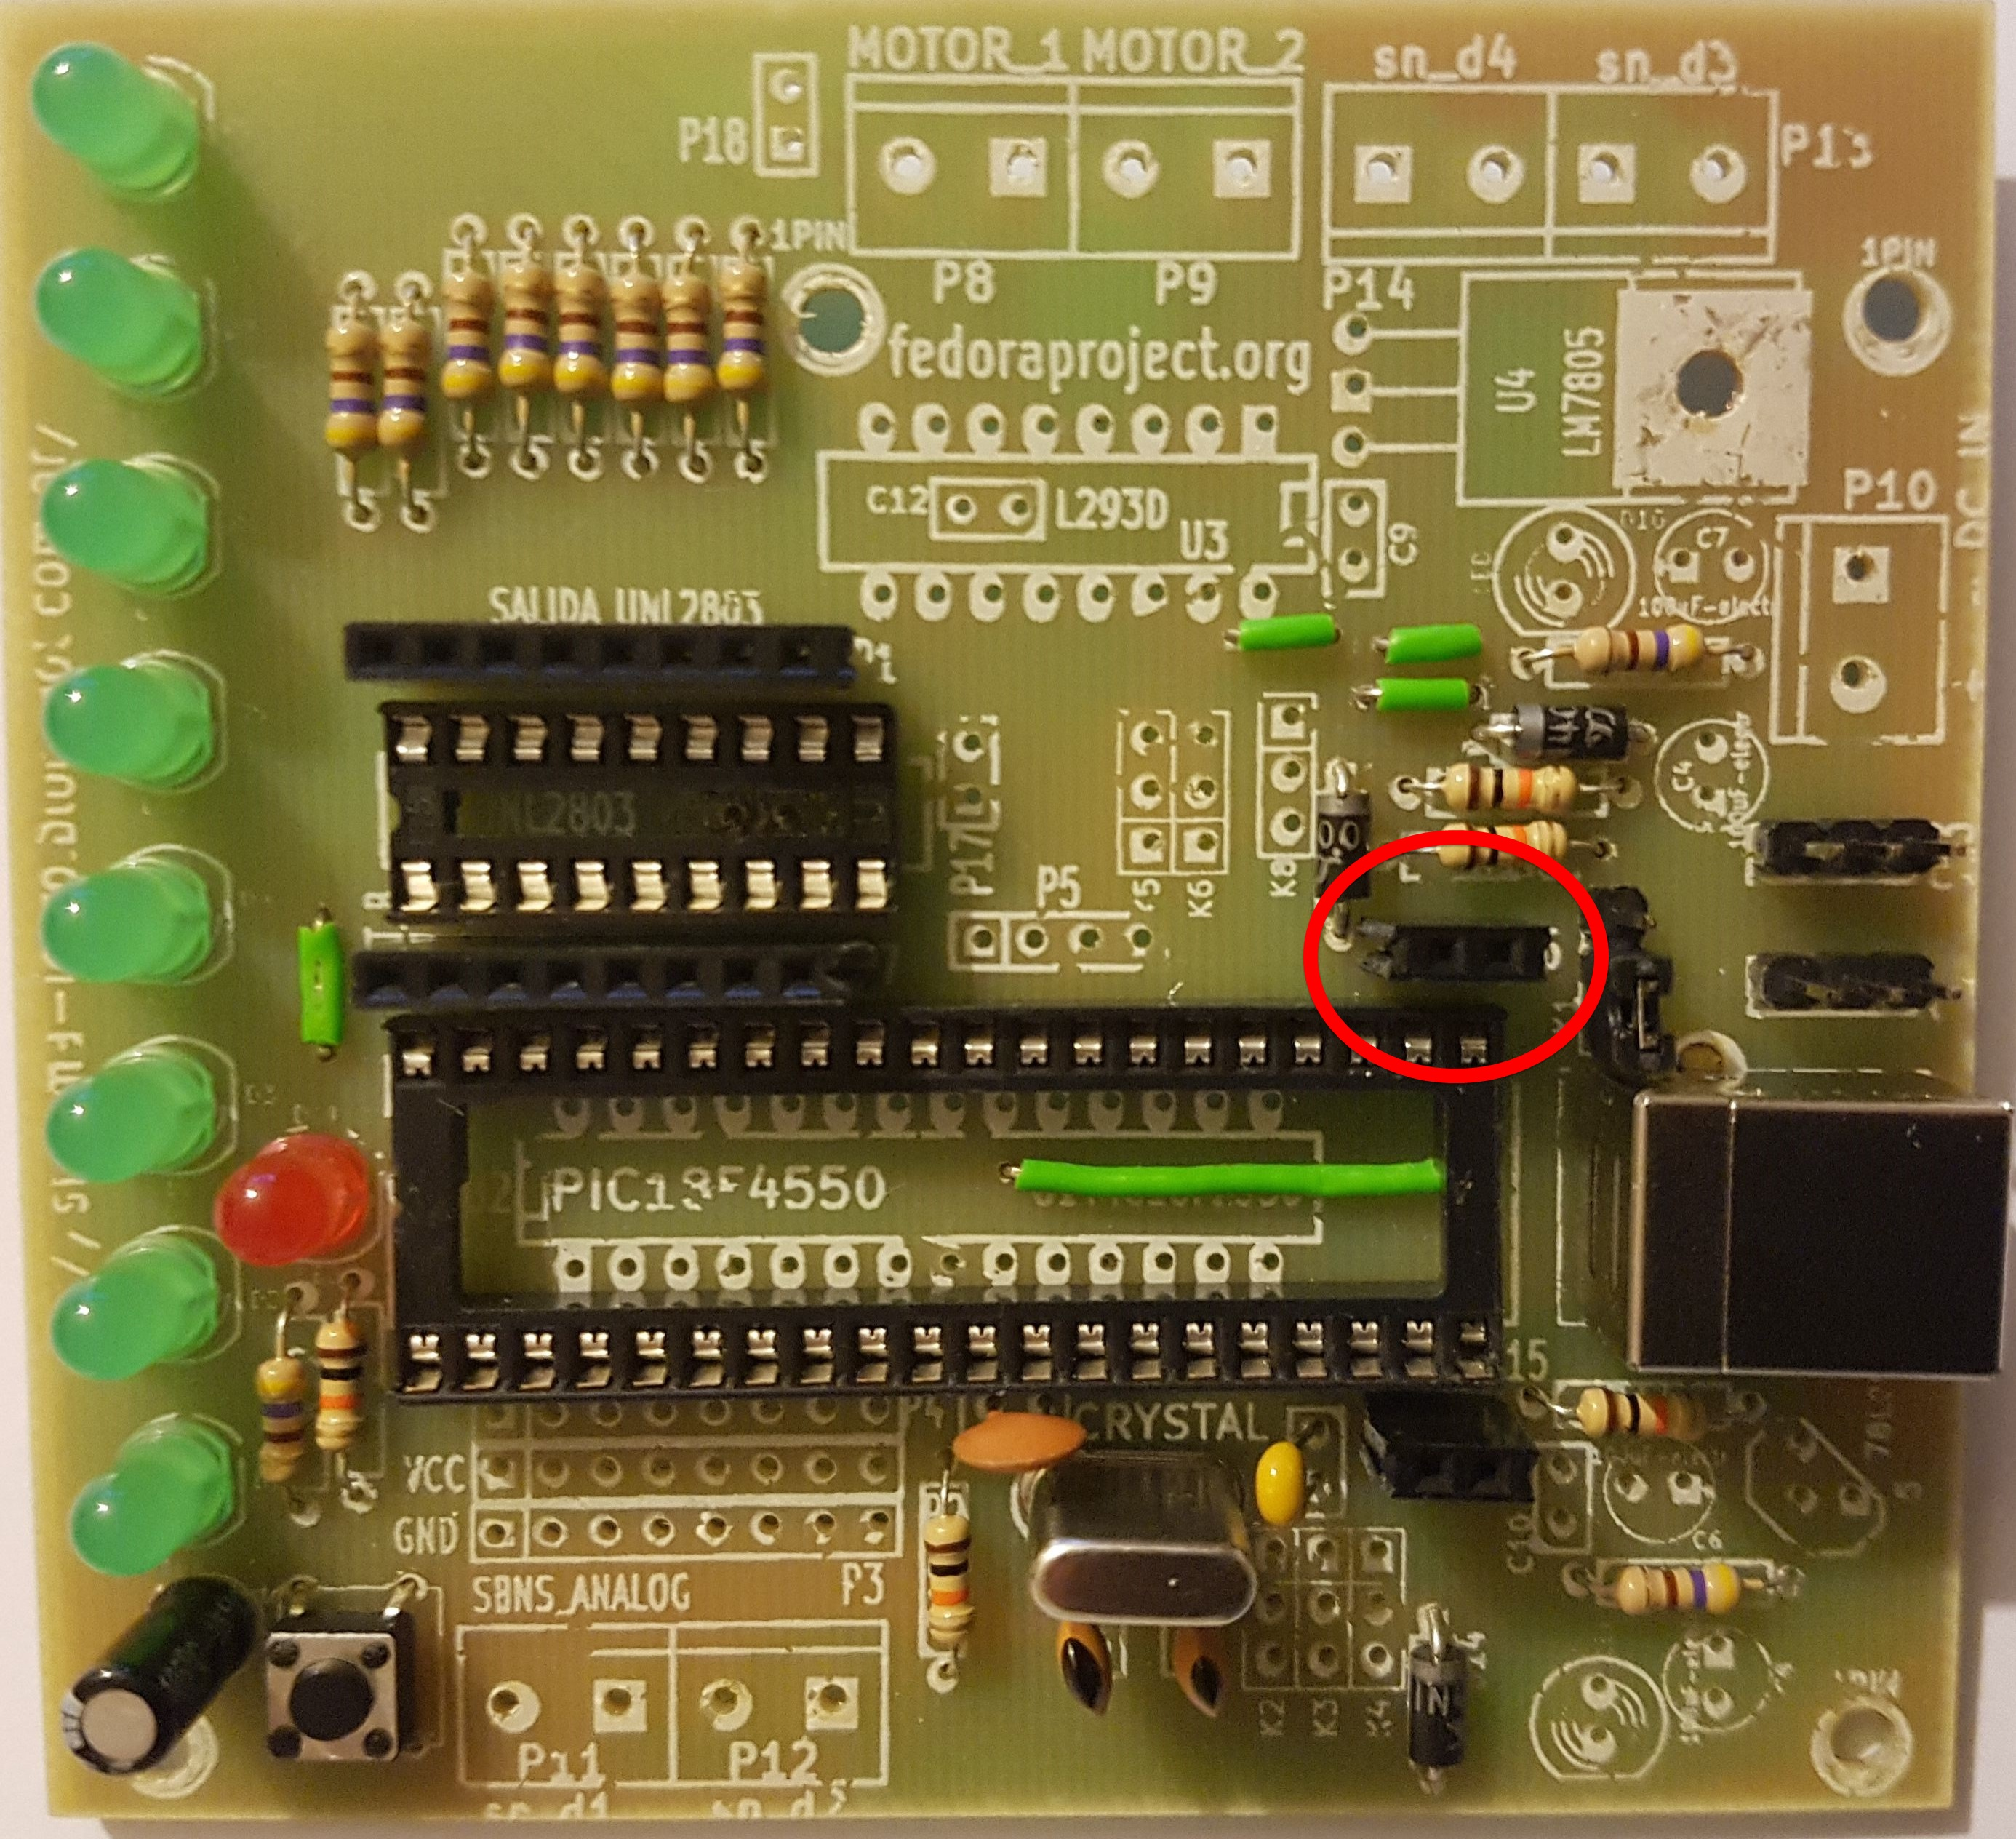
\includegraphics[width=0.8\linewidth]{Modulo_3/M3_8}
	\caption{Módulo 3 - Paso 8}
	\label{fig:M3_8}
\end{figure}

\newpage

\section{Paso 9:}

Instalar borneras de 2 posiciones P11 a P14

\begin{figure}[h]
	\centering
	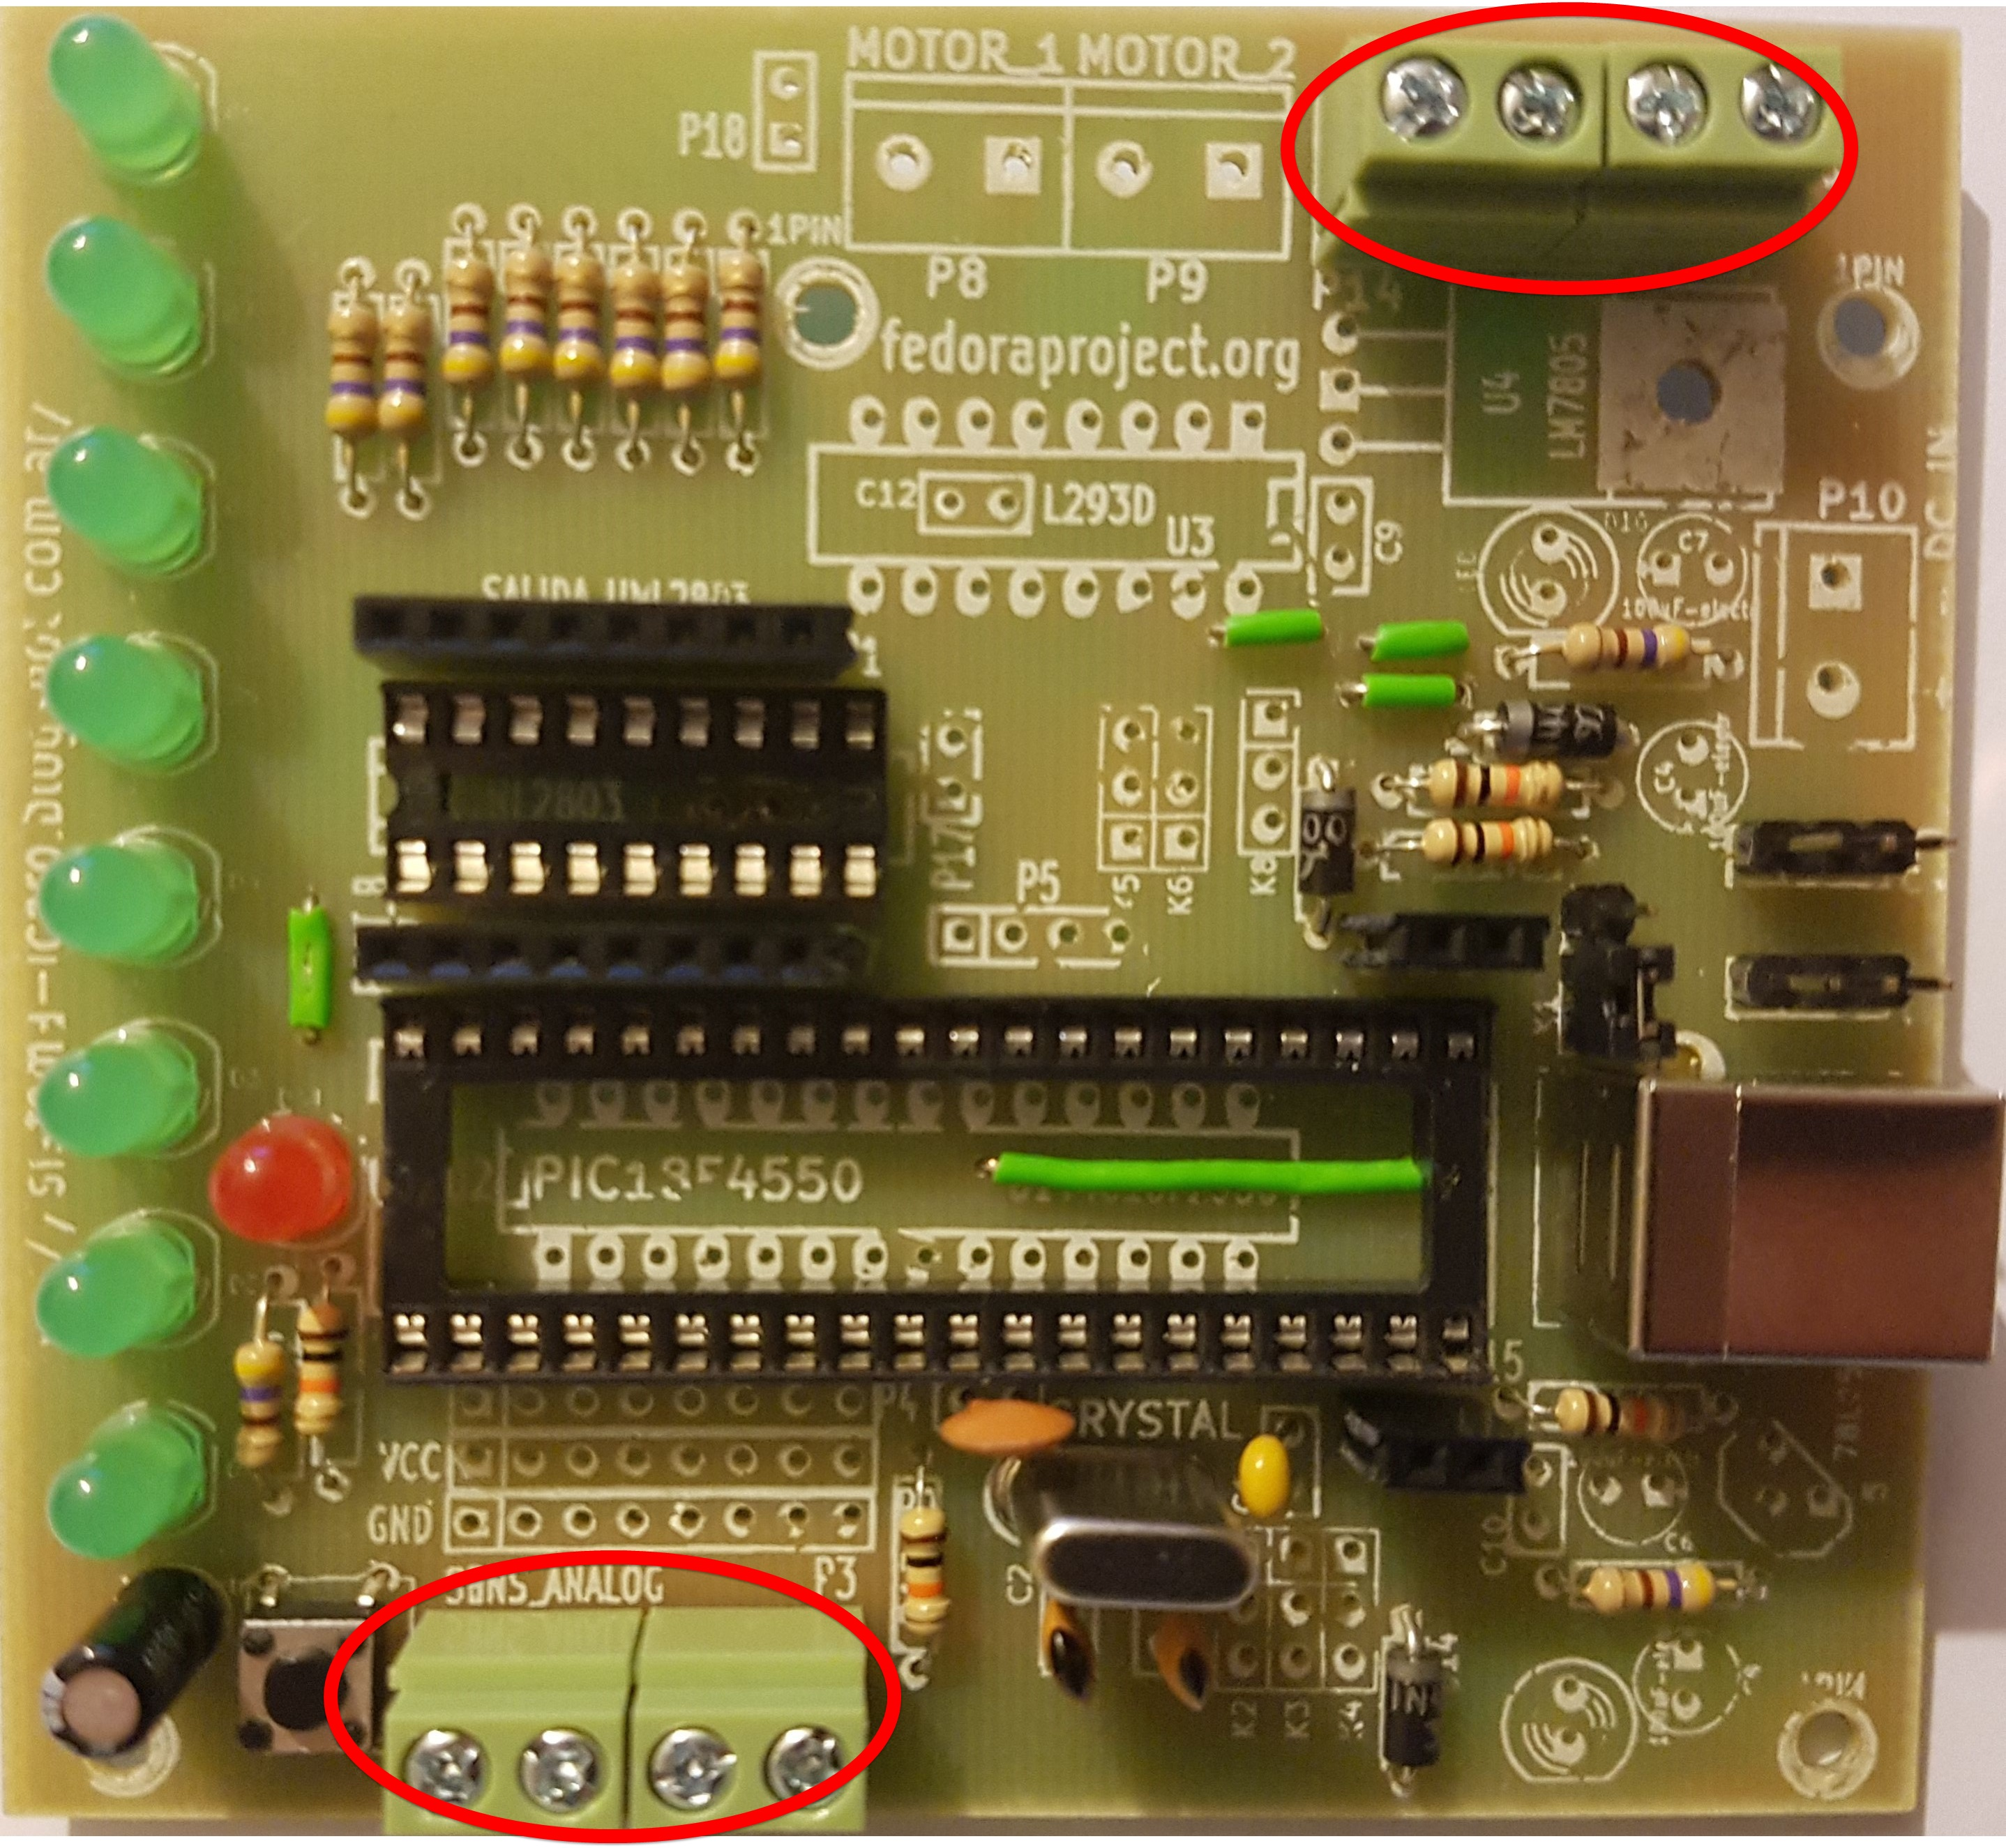
\includegraphics[width=0.8\linewidth]{Modulo_3/M3_9}
	\caption{Módulo 3 - Paso 9}
	\label{fig:M3_9}
\end{figure}

\newpage

\section{Paso 10:}

Instalar UNL2803 en P6

\begin{figure}[h]
	\centering
	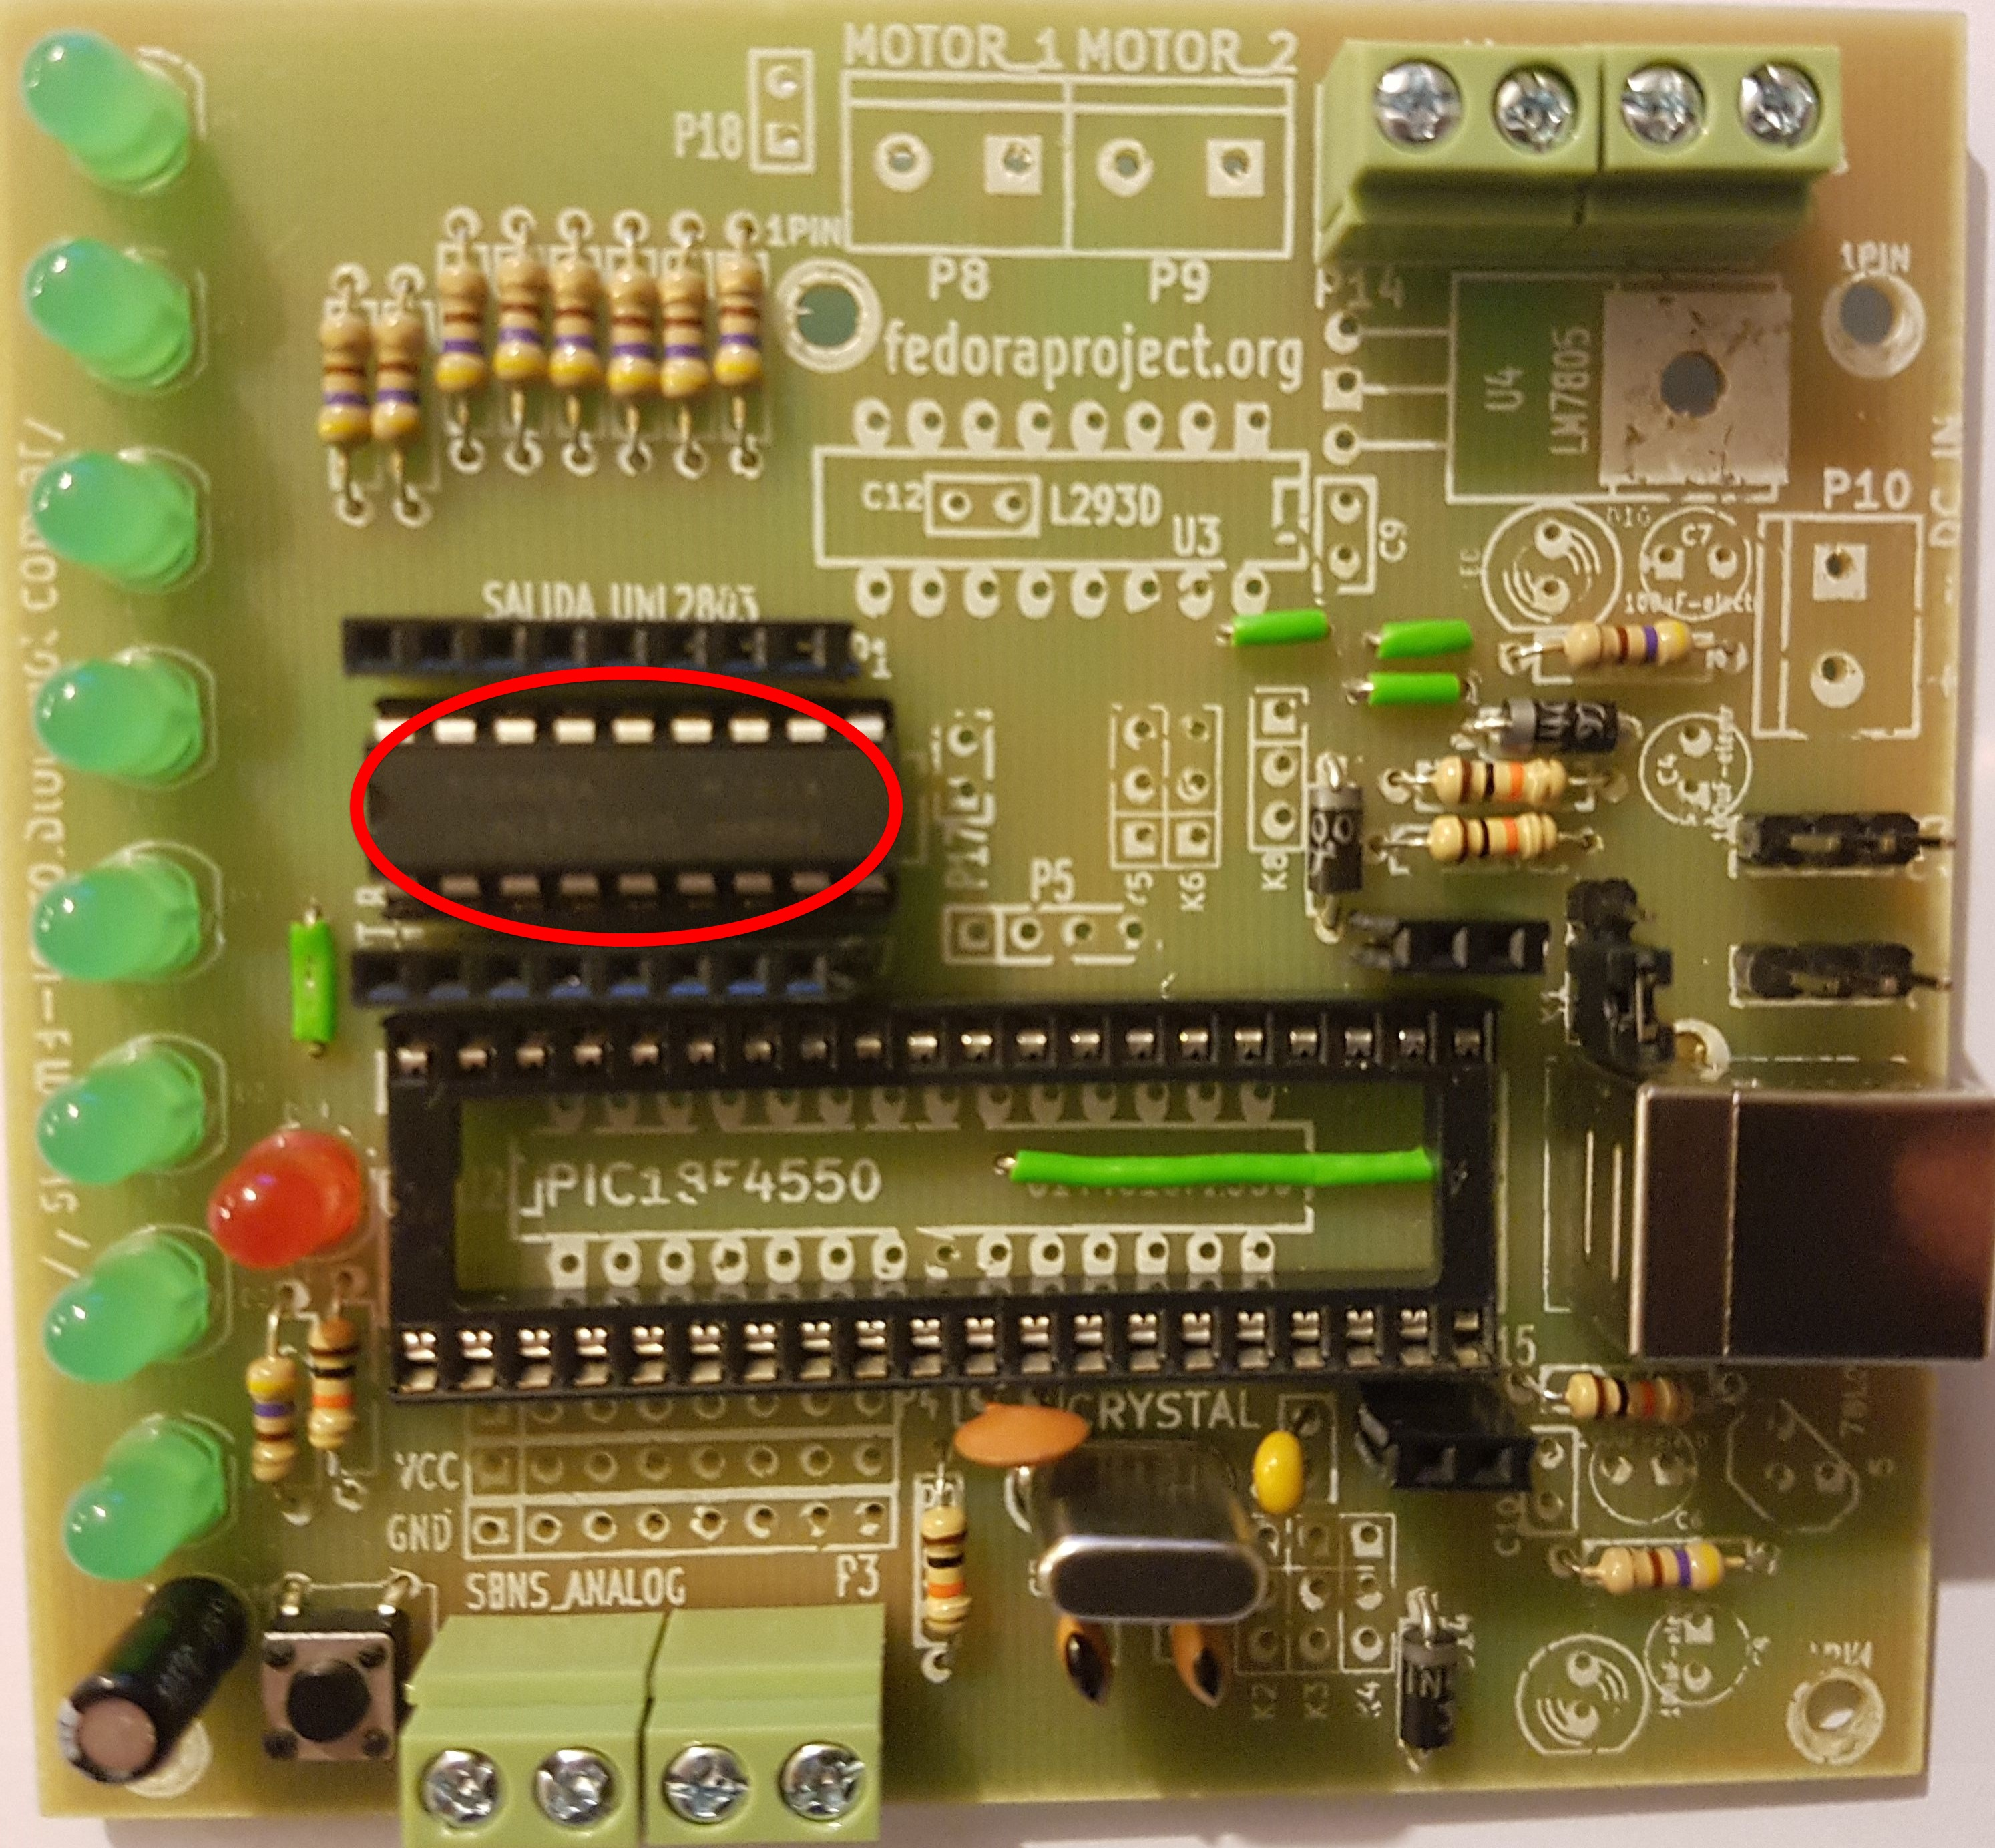
\includegraphics[width=0.8\linewidth]{Modulo_3/M3_10}
	\caption{Módulo 3 - Paso 1}
	\label{fig:M3_10}
\end{figure}

\newpage

Comprobación:
Instalar el microcontrolador si no está instalado.
Cargar un script de ejemplos de la sección de leds y ver si los leds se encienden.
Cargar un script de ejemplos de la sección de icaro testing llamado sensores digitales. Con un cable o alambre, hacer corto entre los polos de la bornera sn-d1 y ver si el led D8 se enciende. Luego hacer corto entre los polos de la bornera sn-d2 y ver si el led D7 se enciende. Luego hacer corto entre los polos de la bornera sn-d3 y ver si el led D6 se enciende. Finalmente hacer corto entre los polos de la bornera sn-d4 y ver si el led D5 se enciende. 

